\documentclass{sig-alternate}

\usepackage{times}
\usepackage{verbatim}
\usepackage{subfigure}
\usepackage{multirow}
\usepackage{url}
\usepackage{color}
\usepackage{balance}
\usepackage{framed}
\makeatletter
\newif\if@restonecol
\makeatother
\let\algorithm\relax
\let\endalgorithm\relax
\usepackage[lined,algonl,boxed]{algorithm2e}%\usepackage{mathbb}

\newcommand{\reminder}[1]{\textbf{\color{red}[** #1 **]}}  % to fix
\newcommand{\hide}[1]{} %hide
\newcommand{\vpara}[1]{\vspace{0.08in}\noindent\textbf{#1 }}
\newcommand{\para}[1]{\vspace{0.01in}\noindent\textbf{#1 }}
\newcommand{\secref}[1]{Section~\ref{#1}} %section reference
\newcommand{\Real}{\ensuremath{\mathbb{R}}}  % Real numbers
\newcommand{\figref}[1]{Figure~\ref{#1}} %section reference
\newcommand{\beq}[1]{\vspace{-0.02in}\begin{equation}#1\end{equation}\vspace{-0.02in}}
\newcommand{\beqn}[1]{\vspace{-0.03in}\begin{eqnarray}#1\end{eqnarray}\vspace{-0.03in}}
\newcommand{\beal}[1]{\vspace{-0.03in}\begin{align}#1\end{align}\vspace{-0.03in}}
\newcommand{\besp}[1]{\begin{split}#1\end{split}}
\newcommand{\remark}[1]{\textbf{\color{red}**#1**}}
%\newcommand{\eeq}[1]{\end{equation}\normalsize}

\newdef{definition}{Definition}
\newdef{problem}{Problem}
\newdef{theorem}{Theorem}
\newtheorem{hypothesis}{Hypothesis}

\newfont{\mycrnotice}{ptmr8t at 7pt}
\newfont{\myconfname}{ptmri8t at 7pt}
\let\crnotice\mycrnotice%
\let\confname\myconfname%


\begin{document}

\title{Null Models For Social Networks}

\numberofauthors{2}
%
% Put no more than the first THREE authors in the \author command

% NOTE: All authors should be on the first page. For instructions
% for more than 3 authors, see:
% http://www.acm.org/sigs/pubs/proceed/sigfaq.htm#a18
\author{
%
% The command \alignauthor (no curly braces needed) should
% precede each author name, affiliation/snail-mail address and
% e-mail address. Additionally, tag each line of
% affiliation/address with \affaddr, and tag the
%% e-mail address with \email.
\alignauthor Jessica Su\\
       \affaddr{Group \#3}\\
       \affaddr{Stanford University}\\
       \email{jtysu@stanford.edu}
\alignauthor Sen Wu\\
       \affaddr{Group \#3}\\
       \affaddr{Stanford University}\\
       \email{senwu@stanford.edu}
}

\maketitle
\begin{abstract}

\end{abstract} 

%\vspace{-0.02in}
% A category with only the three required fields
\category{J.4}{Social and Behavioral Sciences}{Miscellaneous}

%\category{H.4.m}{Information Systems}{Miscellaneous}
%\vspace{-0.08in}
\terms{Algorithms, Experimentation}
%\vspace{-0.08in}
\keywords{Social networks}


\section{Introduction}
\label{sec:intro}

Many real-world systems can be modeled by graphs, from power grids to arXiv citations to friendships on Facebook.  Early models attempted to model all systems with the same type of graph.  For example, the Erdos-Renyi random graph~\cite{erdds1959random}\cite{erdos1960random} models all networks with $n$ participants and $m$ connections with a graph of $n$ nodes and $m$ randomly placed edges.  The Watts-Strogatz model~\cite{watts1998collective} models all networks by connecting nodes to their nearest neighbors, then filling the rest of the graph with randomly placed edges.

More sophisticated models account for differences in degree distribution and clustering coefficient.  The preferential-attachment model~\cite{albert2002statistical} generates a graph with power-law degree distribution and allows the modeler to choose the exponent in the power law.  The configuration model takes as input an exact sequence of degrees and creates a random graph with that degree sequence.  Newman's "triangle-edge" model~\cite{newman2009random} generalizes this to create a random graph with specific degree sequence and clustering coefficient.

Our objective is to create a random graph with specific degree sequence and
motif counts.  (See Figure~\ref{fig:network} for an example of motif
counts.)  A motif is a small, connected subgraph of a larger graph,
and we only consider motifs with four or fewer vertices in our analysis 
(Figure~\ref{fig:motif}).  Motif counts are useful for distinguishing different
types of real-world graphs.  A network like Twitter (when converted to an
undirected graph) might have many Four
Star motifs, since a small fraction of users have large numbers of
followers who do not follow each other.  By contrast, a network like
Facebook would have a disproportionate number of Four Complete motifs, 
since a user's Facebook friends often have many mutual friends with the
user himself.  Finding the motif balance allows us to distinguish
"celebrity-based" networks from "friendship-based" networks.  (There are
also many other types of networks; email forwarding chains would have a
large number of line graphs, as would product recommendation graphs.)

\begin{figure}[t]
\centering
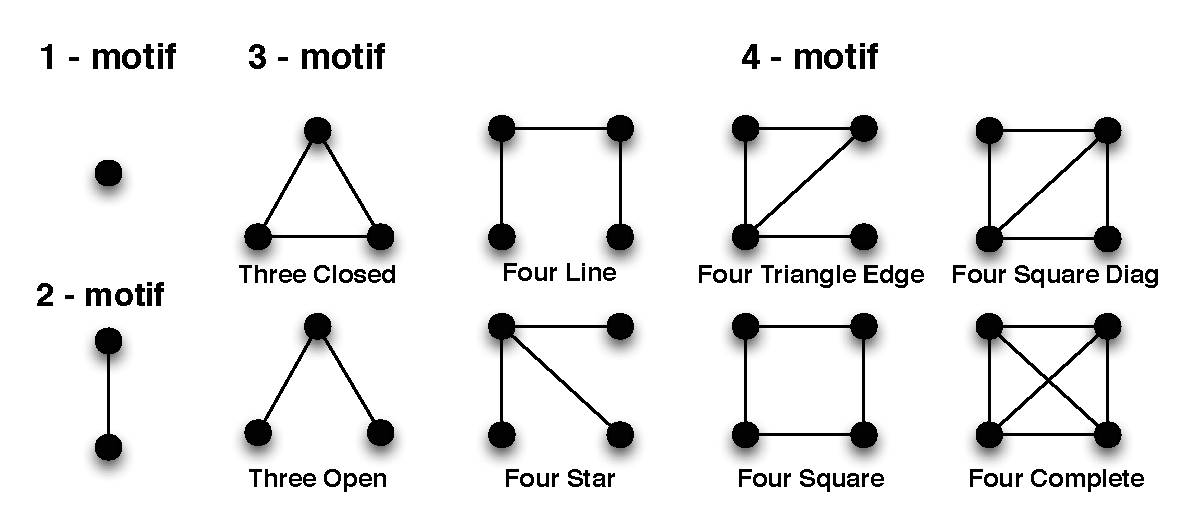
\includegraphics[width=3in]{Figures/motifs1.eps}
\caption{Graphical representation of the motifs.}
\label{fig:motif}
\end{figure}


These structures are not fully captured by models that look only at
3-motifs or clustering coefficients.  Knowing only the number of triangles
(Three Closed) and triads (Three Open), we could not tell the difference
between two strangers with one mutual friend and two strangers with two
mutual friends.  The first might correspond to two people in different
social circles who are both connected to a social "hub," while the
second might correspond to two people in the same class who know
several of the same classmates but have not yet met.  Using 4-motifs gives
us a better sense of the structure of the graph.  While
we might obtain better results by using 5- and 6-motifs, this is more
computationally intensive and we relegate it to future work.

This intuition was formalized by Chuanqi Shen, who built a classifier to
cluster networks according to their motif counts.  He found that the
clusters corresponded closely to real-life functionality~\cite{chuanqi}.
Therefore, by generating graphs with similar motif counts, we hope to build 
graphs with similar function to real-world networks.

\begin{figure}[t]
\centering
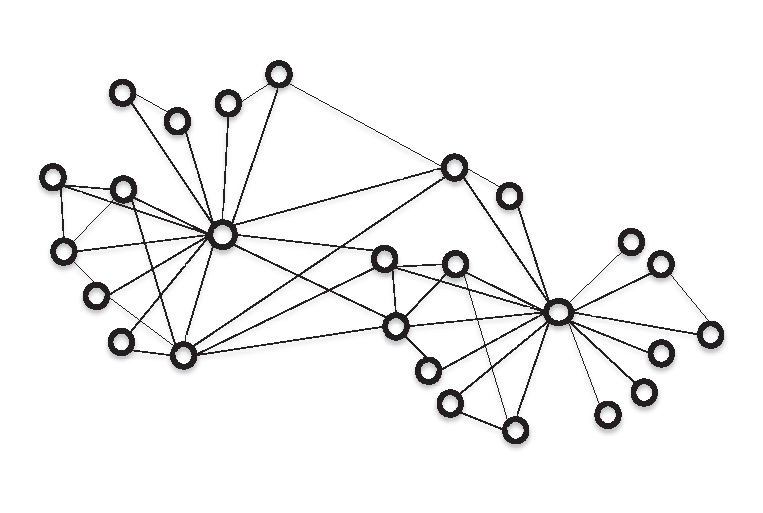
\includegraphics[width=3in]{Figures/network.eps}
\caption{A network with motif distribution \{numNodes: 25, numEdges: 44,
mtThreeClosed: 21, mtThreeOpen: 151, mfFourLine: 134,
mfFourSquare: 1, mfFourStar: 305, mfFourTriangleEdge: 155,
mfFourSquareDiag: 26, mfFourComplete: 2\}.}
\label{fig:network}
\end{figure}

%While it is difficult to find exact solutions, we use hill-climbing to find approximate solutions that produce good results in practice.

The rest of the paper is organized as follow: Section \ref{sec:problem} formulates the problem; Section \ref{sec:related} discusses related work; Section \ref{sec:approach} explains the proposed framework and describes the algorithm for generating random graph; Section \ref{sec:exp} presents the experimental results; finally,  and Section \ref{sec:futurework} concludes the future work.



%\section{Background}
\label{sec:background}

\begin{figure}[t]
\centering
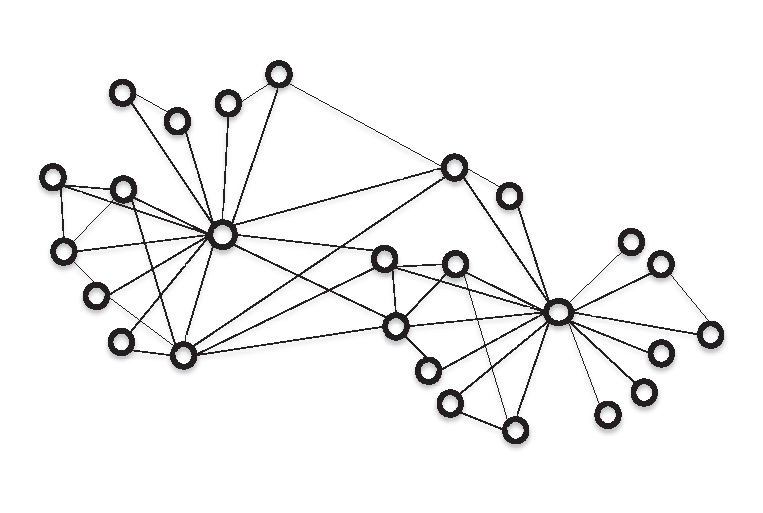
\includegraphics[width=3in]{Figures/network.eps}
\caption{A sample social network.}
\label{fig:network}
\end{figure}

\begin{figure}[t]
\centering
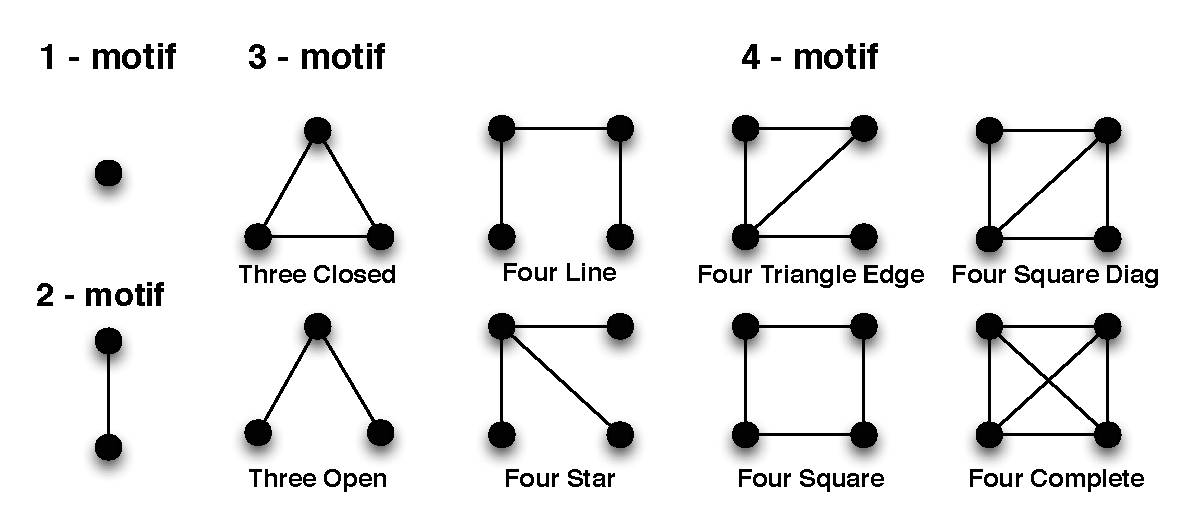
\includegraphics[width=3in]{Figures/motifs1.eps}
\caption{Graphical representation of the motifs.}
\label{fig:motif}
\end{figure}

In this section, we first give some basic concepts that we use throughout the paper. Then, we formulate the problem of motif-driven graph generation. 

A \textbf{graph} is a representation of a set of objects and the
connections between them.  It is defined as a tuple $(V, E)$, where $V$ is
a set of $|V| = N$ vertices ("nodes") and $E \subseteq V \times V$ is a set of edges.
The nodes in a graph correspond to the objects, and the edges to
the connections.

A graph is called \textbf{simple} if no node has an edge to itself and no two
nodes have more than one edge between them.  A graph is \textbf{undirected}
if whenever $(v, w)$ is an edge, $(w, v)$ is also an edge.  In our problem, 
we assume all graphs are simple and undirected.

A \textbf{subgraph} of $G$ is a graph whose nodes and edges form subsets of 
the nodes and edges of the graph $G$.  An
\textbf{induced subgraph} of $G$ on the vertices $V' \subseteq V$ is the
graph consisting of the vertices $V'$ and the edges between them.

A \textbf{motif} is a small, connected graph, often considered as a
subgraph of a larger graph. In this paper, we only
consider motifs within $4$ vertices, which we term "1-motif", "2-motif", "3-motif" and
"4-motif" respectively. Note that, 1-motif is simply a vertex, and 2-motif is simply an edge. A full list of motifs is shown in
Figure~\ref{fig:motif}.

The \textbf{motif distribution} of a graph $G$ specifies how many of each
motif type the graph contains.  For example, in Figure~\ref{fig:network} represents a graph with motif
distribution \{mtThreeClosed: 12, mtThreeOpen: 16, mfFourLine: 22,
mfFourSquare: 18, mfFourStar: 30, mfFourTriangleEdge: 10, mfFourSquareDiag:
17, mfFourComplete: 2\} would contain twelve triangles, two 4-cliques, and
so forth.

\section{Problem Definition}
\label{sec:problem}
Our problem is to generate a network with a specific motif distribution.

\vpara{Input:} A motif distribution $D$, where each motif has at most $4$ vertices.

\vpara{Output:} A graph $G$ with a motif distribution that closely approximates $D$.
\\\\
In this report we focus on an easier problem, where we are given both a motif distribution and the real-life network it corresponds to.  This problem is easier since it allows us to use the degree distribution of the original network.  It also guarantees that a solution exists, which is not true for all motif distributions.  (For example, there are no graphs with two nodes and three triangles.)

If our purpose is to compare null models to real data sets, it suffices to solve the easier problem, since we have the data required to create the model.  However, in the final report, we will extend our solution to solve the harder problem.

%The problem formulation is different from other graph generation problems
%\cite{erdds1959random, watts1998collective, albert2002statistical,
%newman2009random, molloy1995critical}, as in this paper we focus on
%generating graphs based on the motif distribution.
%Motif distributions are frequently used for analyzing large graphs in the
%social sciences.

\section{Related work}
\label{sec:related}

\vpara{Motif} Graph motif is an important local property which are defined as recurrent and statistically significant subgraph or patterns. Many research related to graph motifs. 
Shen-Orr et al.~\cite{shen2002network} present new algorithms for systematically detecting network motifs to one of the best-characterized regulation networks, that of direct transcriptional interactions in Escherichia coli. 
Milo et al.~\cite{milo2002network} use the network motif to uncover the complex networks structural design principles.
Alon et al.~\cite{alon2007network} review network motifs and their functions, with an emphasis on experimental studies.
Recently, Bhuiyan et al.~\cite{bhuiyan2012guise} propose a method called \textit{GUISE}, which uses a Markov Chain Monte Carlo (MCMC) sampling method for constructing the approximate GFD\footnote{Graphlet frequency distribution, Graphlet is also called motif} of a large network.

\vpara{Generating random graph} Generating random is an important problem in social network analysis. 

Most research is to generate random graph based on degree. 
Molloy et al.~\cite{molloy1995critical} provide a model for generating random graphs with given degree sequence. 
Rao et al.~\cite{rao1996markov} propose an MCMC based model using switches along alternating cycles for generating random. 
Bayati et al.~\cite{bayati2010sequential} present a nearly-linear time algorithm for counting and randomly generating simple graphs with a given degree sequence in a certain range. 
Milo et al.~\cite{milo04random} propose a approach for generating a random graph with prescribed degree sequence. Our approach inspired by Milos's and it begins by generating an arbitrary graph with that degree sequence.  (This can be done by giving each node a certain number of ``half-edges,'' then connecting them randomly to form the edges of the graph.)  One this graph is generated, he chooses pairs of edges at random and swaps the endpoints, repeating this step until the graph is sufficiently ``randomized.''

\begin{algorithm}
\caption{Milo's approach for generating random graphs with prescribed degree sequences.}
\label{algorithm:milo}
\begin{algorithmic}
Generate graph $G = (V, E)$ with required degree sequence\\
\While{Markov chain displays insufficient mixing}{
    Choose $e_1, e_2 \in E$ at random\\
    Add edges $(e_1.Src, e_2.Dst)$, $(e_2.Src, e_1.Dst)$\\
    Delete edges $(e_1.Src, e_1.Dst)$, $(e_2.Src, e_2.Dst)$\\
}
\end{algorithmic}
\end{algorithm}

This ``rewiring'' step is innovative because it preserves both the number of edges and the degree of each node.  For this reason we use the same rewiring step in our algorithm.

\hide{

Our approach is inspired by Milo's approach for generating a random graph with prescribed degree sequence.~\cite{milo04random} He begins by generating an arbitrary graph with that degree sequence.  (This can be done by giving each node a certain number of ``half-edges,'' then connecting them randomly to form the edges of the graph.)  One this graph is generated, he chooses pairs of edges at random and swaps the endpoints, repeating this step until the graph is sufficiently ``randomized.''

\begin{algorithm}
\caption{Milo's approach for generating random graphs with prescribed degree sequences.}
\label{algorithm:milo}
\begin{algorithmic}
Generate graph $G = (V, E)$ with required degree sequence\\
\While{Markov chain displays insufficient mixing}{
	Choose $e_1, e_2 \in E$ at random\\
	Add edges $(e_1.Src, e_2.Dst)$, $(e_2.Src, e_1.Dst)$\\
	Delete edges $(e_1.Src, e_1.Dst)$, $(e_2.Src, e_2.Dst)$\\
}
\end{algorithmic}
\end{algorithm}

This ``rewiring'' step is innovative because it preserves both the number of edges and the degree of each node.  For this reason we use the same rewiring step in our algorithm.
}
%\section{Hardness of Problem}
\label{sec:nphard}

In this section, we describe the difficulty of the exact motif generation problem.


Given the definition of problem, the motif-driven graph generation problem can be cast as nonlinear programming problem. Let $X_{ij}$ denote the existence of the edge $(v_i, v_j)$ in graph, where $X_{ij} = 1$ if edge $(i, j)$ is in graph, $0$ otherwise. With the motifs can be represent by a polynomial combination of $X_{ij}$, for example, Three Closed of nodes $v_a, v_b, v_c$ as $X_{ab}X_{bc}X_{ac}$ and Four Triangle Edge of $v_a, v_b, v_c, v_d$ as $X_{ab}X_{bc}X_{ca}X_{ad}(1 - X_{bd})(1 - X_{cd})$. For each kind of motif, we can build a nonlinear function to represent the number of motif. Then, we can construct a nonlinear equations.

\theorem The problem of motif generate grpah by $k$-motif is NP-hard, even in the case of there is only triangle closed motif.

\Proof In the case of triangle closed motif, the problem can be reduced to $min\{\sum_{i,j,k} X_{ij}X_{jk}X_{ki}\}, X_{ij} \in \{0, 1\}$, which is an typical nonlinear integer programming. And the problem can further equal to
\begin{align*}
\min\mbox{ }&C\\
s.t. &\sum_{i,j,k} X_{ij}X_{jk}X_{ki} \leq C\\
&X \geq 0, X \in \{0, 1\}^n
\end{align*}

According to R. Hemmecke's~\cite{hemmecke2009nonlinear} theory, $\sum_{i,j,k} X_{ij}X_{jk}X_{ki} \leq C$ can be transfer to the linear function, which means the problem equals to the a special case of  linear programming which is 0-1 integer linear programming. This problem is known to be NP-complete. This is one of Karp's 21 NP-complete problems; \cite{karp1972reducibility} Karp showed the NP-completeness by a reduction from the vertex cover problem. So, our motif generation is also NP-complete.

%\section{Data and Observations}
\label{sec:observations}

\section{Our Approach}
\label{sec:approach}

In this section, we present a approach framework for generating the graph. At the high level, our proposed framework consists of two stage.
\begin{itemize}
    \item {\bf Degree distribution generation.} First, given a certain motif distribution, we train a gradient boosting model using the motif distribution. And then we predict the degree distribution from motif distribution.
    \item {\bf Candidate graph generation.} Second, with the degree distribution, we generate a random graph based on degree distribution as candidate graph for our problem.
    \item {\bf Graph refinement.} Second, the random graph is fed to a heuristic model to refine the graph. The model incorporates the several strategies to refine the graph satisfied the given motif distribution.
\end{itemize}

\subsection{Degree distribution generation} 

For a given motif distribution, we use the motif distribution to predict degree distribution. The idea of this problem is using the motif distribution as a feature to train a model, and then predict a degree distribution for the given motif distribution. More precisely, we use gradient boosting as the main regression method to train a model. Gradient Boosting Tree~\cite{friedman2002stochastic} is a useful machine learning method for regression problems, which also an ensemble method with combine multiple weak prediction models. It makes the model in a stage-wise fashion and generalizes the model by optimization of the arbitrary differentiable loss function which is same as logistic regression. Here we use the python package build in~\cite{pedregosa2011scikit}. Our approach shows good performance. We achieved less than 1\% on Average Relative Error.

\subsection{Candidate graph generation}

According the degree distribution we got at stage 1, we use 


=======================================

In this section, we propose a heuristic method for generating the required
graph.

\subsection{Hill climbing}
Hill-climbing is a standard technique for finding good solutions to optimization problems.  Start with a solution that is not particularly good.  At each step, perturb the solution randomly.  If the new answer is better, keep it; if not, keep the old solution.  Repeat this until the algorithm converges to a good solution.

Hill-climbing does not guarantee an optimal solution, since it tends to get stuck at local maxima.  Yet in practice the solutions it finds are "pretty good," especially after running the algorithm several times and picking the best solution.

In our case we minimize the error between the desired motif counts and our solution's motif counts:
\begin{equation}
\label{eqn:avgRelativeError}
\mbox{Average relative error} = \frac{1}{\ell} \sum_{i = 1}^{\ell} \frac{|\mbox{counts}_i - \widehat{\mbox{counts}}_i| + 1}{|\mbox{counts}_i| + 1}
\end{equation}
where $\ell$ is the number of different motif types.

We use the configuration model to generate a random graph with the required degree sequence.  Then at each step we choose two edges (at random) and swap their endpoints.  We count the motifs and compare the error with the new counts to the error with the old counts.  If the new counts give a smaller error, we keep the new graph; otherwise, we discard it.

\begin{algorithm}
\caption{Naive approach}
\label{algorithm:naive}
\begin{algorithmic}
Initialize graph $G = (V, E)$ with prescribed degree sequence\\
motifCounts <- CountMotifs($G$)\\
\Repeat{computation time limit exceeded} {
	Choose $e_1, e_2 \in E$ at random\\
	Add edges $(e_1.Src, e_2.Dst)$, $(e_2.Src, e_1.Dst)$\\
	Delete edges $(e_1.Src, e_1.Dst)$, $(e_2.Src, e_2.Dst)$\\
	newMotifCounts <- CountMotifs($G$)\\
	\eIf {error(newMotifCounts) < error(motifCounts)} {
		motifCounts <- newMotifCounts\\
	} {
		Return graph to original state\\
	}
}

\end{algorithmic}
\end{algorithm}

\subsection{Optimizations}
As written, this solution is very slow.  Counting motifs is $O(|V|^4)$ and takes unacceptably long in practice.  To get good results in practice, we need a large number of rewiring steps, so ideally each rewiring step should take less than a second.

We can speed this up by counting motifs incrementally.  Instead of considering the whole graph on every step, we only look at the part of the graph whose motifs would be affected by the edge changes.  Since we are only looking at motifs with fewer than $5$ nodes, we can only consider the nodes that are one or two hops away from the nodes whose edges are being rewired.  Then we can count how many motifs are being created or destroyed in the induced subgraph on those nodes, and add those to the total motif counts.  Once we have the induced subgraph, we count the motifs by taking all possible sets of four vertices, and seeing which motif they form, if any.

(In our algorithm we break the rewiring step into four steps, two edge deletions and two edge creations.  This way we only measure the effect of one edge creation/deletion step at a time.)

This is still fairly slow, so we apply one final optimization.  We notice that for a 4-motif to be affected by the edge changes, vertices $1$ and $2$ of the motif must be endpoints of the edge.  Vertex $3$ must be an immediate neighbor of an endpoint, and vertex $4$ is either an immediate neighbor or a second-degree neighbor.  Ordinarily, we would have to loop through the immediate neighbors to find all possibilities for vertex $3$, and perform an inner loop through the second degree neighbors to find all possibilities for vertex $4$.  But if vertex $4$ was always an immediate neighbor, we could loop through the immediate neighbors both times, which would speed up the algorithm considerably.

Vertex $4$ is not always an immediate neighbor of vertex $1$ or vertex $2$.  However, when it's not an immediate neighbor of either endpoint, we can do a lot less computation than we would have to otherwise.  We can break these situations up into three cases:

\begin{figure}
\centering
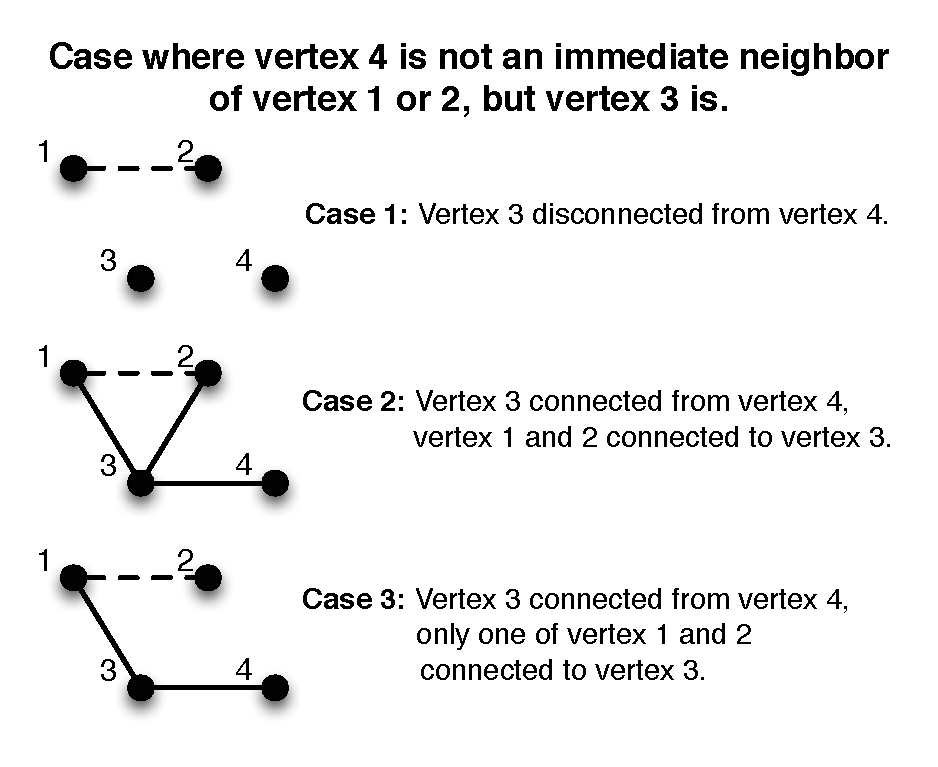
\includegraphics[width=3in]{Figures/case1.eps}
\label{fig:case}
\end{figure}

\begin{itemize}
\item Vertex $3$ is not connected to vertex $4$.  In this case, the four vertices can never form a 4-motif, regardless of whether vertices $1$ and $2$ are connected, and we don't have to change the motif counts.
\item Vertex $3$ and $4$ are connected, and vertex $1$ and $2$ are both connected to vertex $3$.  In this case, connecting vertex $1$ and $2$ deletes a four-star motif and adds a triangle-with-edge motif.
\item Vertex $3$ and $4$ are connected, and only one of vertex $1$ and $2$ are connected to vertex $3$.  In this case, connecting vertex $1$ and $2$ creates a four-line motif.
\end{itemize}

It is much faster to test for these cases than to do the normal
computations (which would involve finding the induced subgraph on those
four vertices, then testing it to see if it was either of the 4-motifs).
So implementing this optimization produces an enormous speedup, allowing us
to perform several thousand rewiring steps in one day.  Each rewiring step
is $O((d_1 + d_2)^2)$, where $d_1$ is the degree of vertex $v_1$, $d_2$
is the degree of vertex $v_2$, and $d_1 + d_2$ is an upper bound on the 
number of first-degree neighbors of $v_1$ and $v_2$.

\subsection{Random restarts}

Hill climbing is an imperfect solution since it is easy to get stuck at
local minima.  We fix this with the method of random restarts.  When we
reach a local minimum, we save the graph and begin rewiring edges randomly.
After this we run hill climbing until we reach another local minimum, then 
repeat the process.  At the end of the computation we return the graph with
lowest error.

We assume the algorithm has reached a local minimum if we have gone through
$|E|$ consecutive rewiring steps without changing the graph.  At this
point, we rewire $|E|/8$ edge pairs randomly and proceed with hill
climbing.  Preliminary results for this approach are presented in 
Section~\ref{sec:exp}.

\section{Experimental Results}
\label{sec:exp}

We conduct various experiments to evaluate our proposed method.
%The datasets are publicly available at the SNAP website.\footnote{http://snap.stanford.edu/data/index.html}

\subsection{Experimental Setup}

\begin{table}[t]
\centering
\begin{tabular}{|c|c@{ }|c@{ }|}
\hline
Dataset             &   \#nodes       &   \#edges \\ \hline
aut-as19971108 & 3015 & 5156 \\\hline
aut-as19990628 & 5322 & 10163 \\\hline
cit-scimet & 3085 & 13474 \\\hline
col-ca-GrQc & 5242 & 14484 \\\hline
col-netscience & 1461 & 2742 \\\hline
met-HI & 1424 & 3423 \\\hline
ppi-ppiall & 3258 & 12930 \\\hline
ppi-ppiapms & 1622 & 9070 \\\hline
pwr-power & 4941 & 6594 \\\hline
\end{tabular}
\caption{Statistics of the nine networks.}
\label{tb:statistics}
\end{table}


\vpara{Data sets.} We evaluate the proposed method on nine different networks: aut-as19971108, aut-as19990628, cit-scimet, col-ca-GrQc, col-netscience, met-HI, ppi-ppiall, ppi-ppiapms and pwr-power.
Table \ref{tb:statistics} lists statistics of the nine networks.  All data was obtained from Jure Leskovec at Stanford University.

\vpara{Evaluation metrics.} To quantitatively evaluate the proposed model, we use the average relative error between the model's motif counts and the motif counts of the real network.  The average relative error is defined in equation~\ref{eqn:avgRelativeError}.

All code is implemented in C++ and Python, and all the evaluations are performed on an x64 machine with Xeon E7-8837 CPU (with 64 cores) and 1024GB RAM. The operating system is CentOS 6. 

\subsection{Performance Analysis}

Hill climbing produces excellent results on most networks.  Table ~\ref{table:errors} shows the improvements in the error after running hill climbing for 24 hours.

Although performance varies across networks, we get at least a 50\% decrease in error for all networks except aut-as19990628 and cit-scimet.  For some networks we get an enormous reduction in error; pwr-power gives a 99.5\% reduction and met-HI gives a 99.9\% reduction.  The first group of figures plots the error over time and the second group plots the probability that a rewiring step will be successful (i.e. that the changes are accepted instead of discarded).

The error graphs for aut-as19971108 (Figure~\ref{fig:errors-aut-as19971108}) and col-netscience (Figure~\ref{fig:errors-col-netscience}) converge to an asymptote.  This indicates that running the procedure longer would not improve the error and the final error is a good reflection of the algorithm's performance.  Since the errors approach nonzero values (and we know a perfect solution exists), this implies that our hill climbing algorithm has found a local minimum.

The graph for pwr-power (Figure~\ref{fig:errors-pwr-power}) rapidly decreases to zero.  This means we have found a perfect or near-perfect solution.  The graph for met-HI (Figure~\ref{fig:errors-met-HI}) also appears to decrease to zero, but that's just because the error started out very high.  (The initial error was 8039.58 and the final error was 0.46768.)

The other error graphs have not yet converged and are steadily decreasing 24 hours after the computation.  This indicates that we can reduce the final error by increasing the computation time and our current results are not a hard limit on the algorithm's performance.

In order to quantify the algorithm's convergence, we plotted the successful rewiring probability over time.  This is the probability that rewiring two edges produces a graph with smaller error than the previous graph.  When this probability reaches zero, the hill climbing algorithm has found a local minimum and cannot proceed further.

The probability curves for pwr-power (Figure~\ref{Paccept-pwr-power}) and col-netscience (Figure~\ref{Paccept-col-netscience}) quickly drop to zero, indicating that the algorithm has converged.  The curves for cit-scimet (Figure~\ref{Paccept-sci-scimet}) and aut-as19990628 (Figure~\ref{Paccept-aut-as19990628}) remain high throughout the algorithm, indicating that we need to run the algorithm longer.  The other curves do not drop to zero, but hover at small nonzero values.  This means the algorithm has not yet converged, but running it longer may yield diminishing returns.

\begin{table*}[t]
\centering
\begin{tabular}{| l | l | l | | l | l | l |}
\hline
Network & Nodes & Edges & Initial error & Final error & Successful rewires\\ \hline
aut-as19971108 & 3015 & 5156 & 0.34216 & 0.16717 & 2951.00\\\hline
aut-as19990628 & 5322 & 10163 & 0.31571 & 0.17723 & 3397.28\\\hline
cit-scimet & 3085 & 13474 & 0.83063 & 0.73247 & 1921.71\\\hline
col-ca-GrQc & 5242 & 14484 & 2.05549 & 0.93973 & 40583.8\\\hline
col-netscience & 1461 & 2742 & 3.13864 & 0.55110 & 8290.71\\\hline
met-HI & 1424 & 3423 & 8039.58 & 0.46768 & 5703.57\\\hline
ppi-ppiall & 3258 & 12930 & 1.06249 & 0.46058 & 38131.1\\\hline
ppi-ppiapms & 1622 & 9070 & 1.37580 & 0.54219 & 24581.7\\\hline
pwr-power & 4941 & 6594 & 0.57996 & 0.00282 & 9485.4\\\hline
\end{tabular}
\caption{Improvements in error after running hill climbing for 24 hours.  All numbers are averaged over $7$ trials.}
\label{table:errors}
\end{table*}

\begin{figure}[p]
\centering
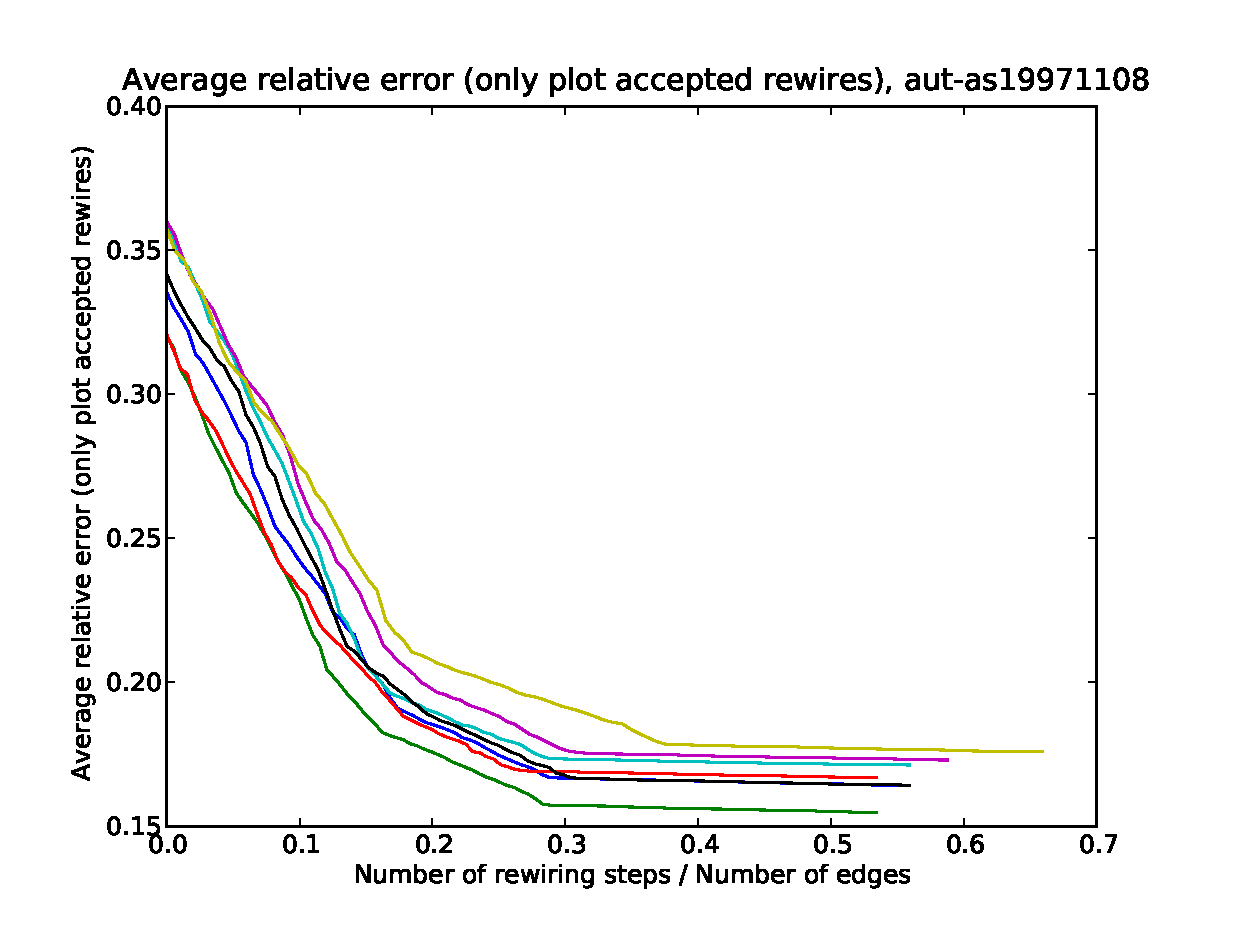
\includegraphics[width=3in]{Figures/acceptedOnly-aut-as19971108.eps}
\caption{Error, network aut-as19971108.  Only plot hill climbing steps that were successful.}
\label{fig:errors-aut-as19971108}
\end{figure}

\begin{figure}[p]
\centering
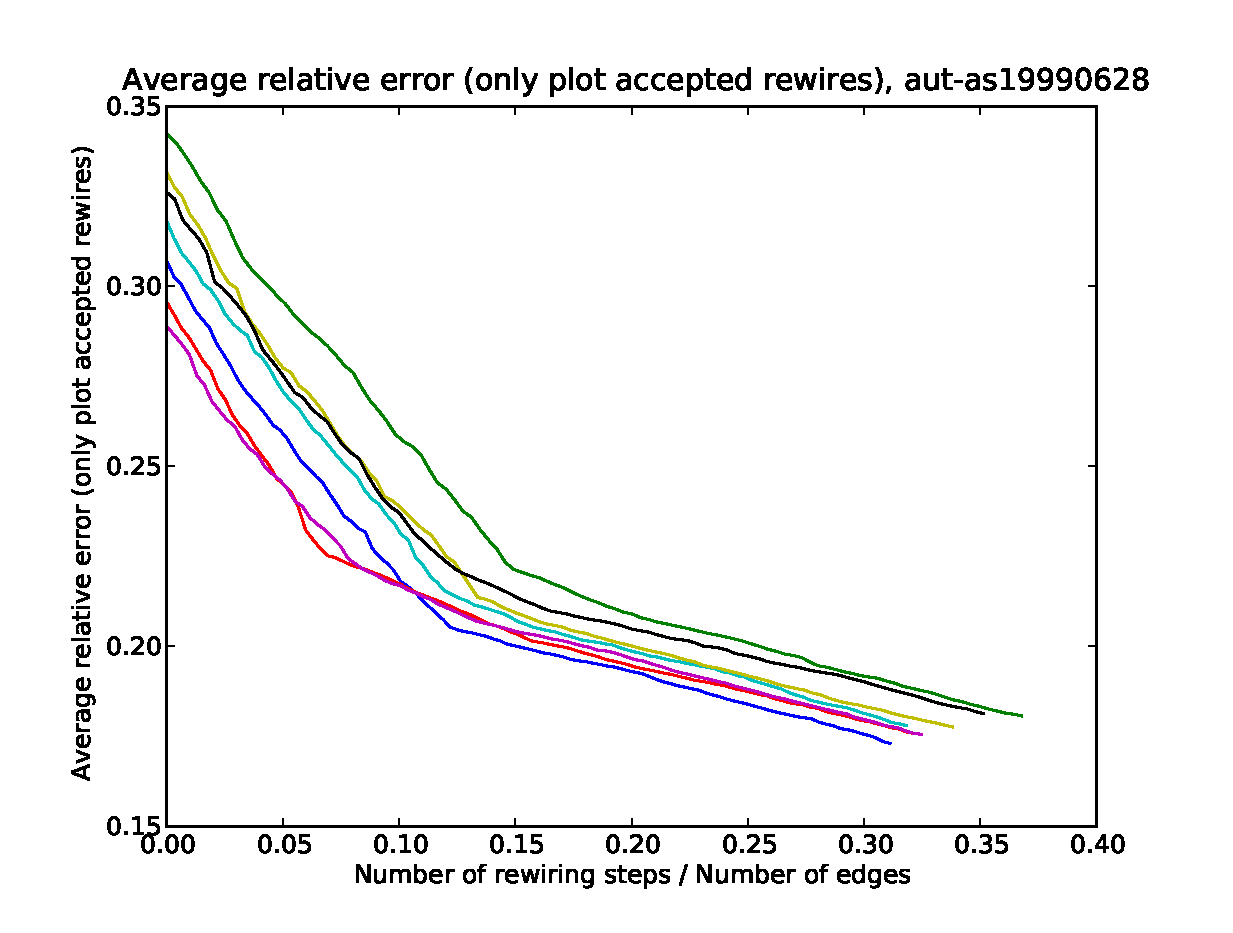
\includegraphics[width=3in]{Figures/acceptedOnly-aut-as19990628.eps}
\caption{Error, network aut-as19990628.  Only plot hill climbing steps that were successful.}
\label{fig:errors-aut-as19990628}
\end{figure}

\begin{figure}[p]
\centering
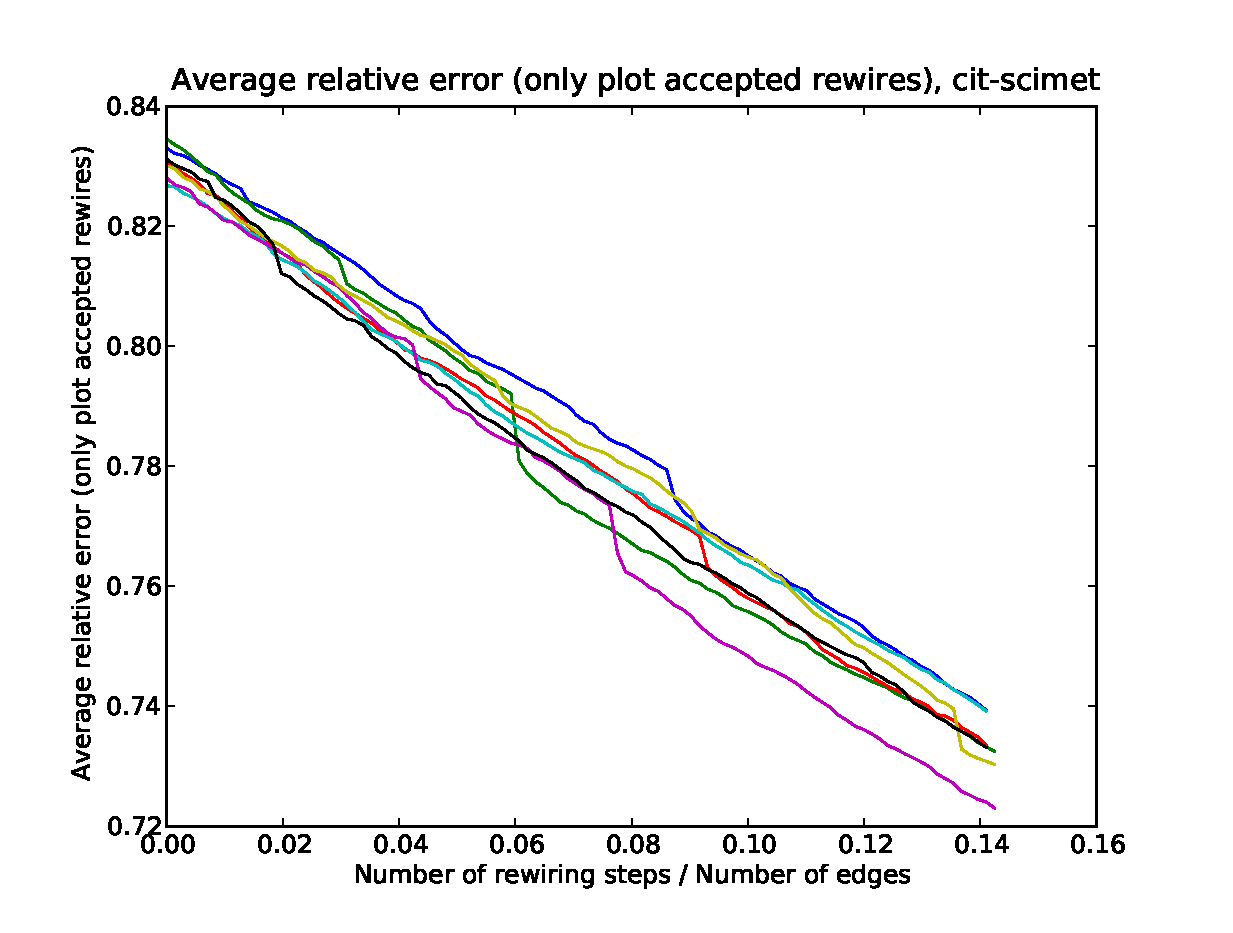
\includegraphics[width=3in]{Figures/acceptedOnly-cit-scimet.eps}
\caption{Error, network cit-scimet.  Only plot hill climbing steps that were successful.}
\label{fig:errors-cit-scimet}
\end{figure}

\begin{figure}[p]
\centering
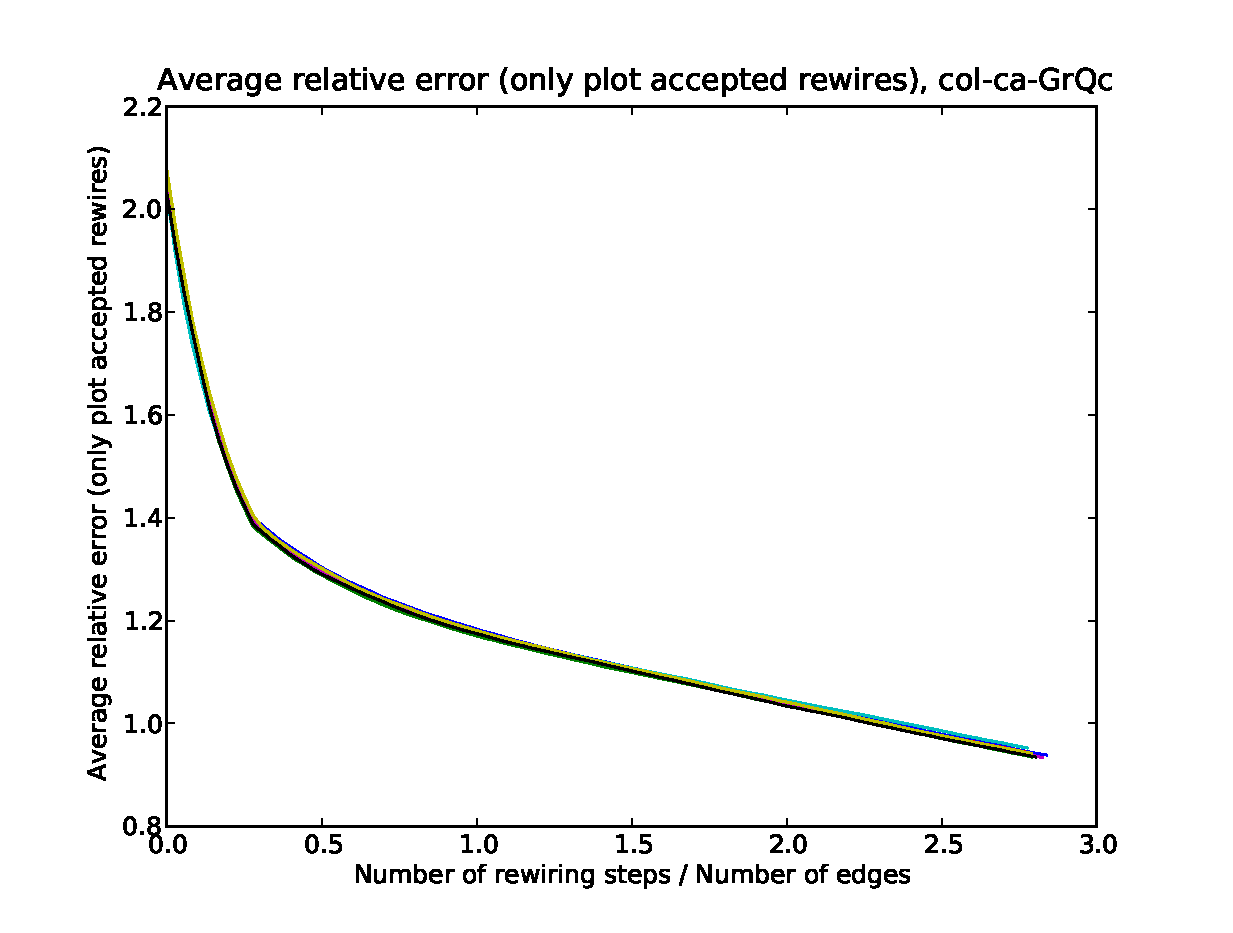
\includegraphics[width=3in]{Figures/acceptedOnly-col-ca-GrQc.eps}
\caption{Error, network col-ca-GrQc.  Only plot hill climbing steps that were successful.}
\label{fig:errors-col-ca-GrQc}
\end{figure}

\begin{figure}[p]
\centering
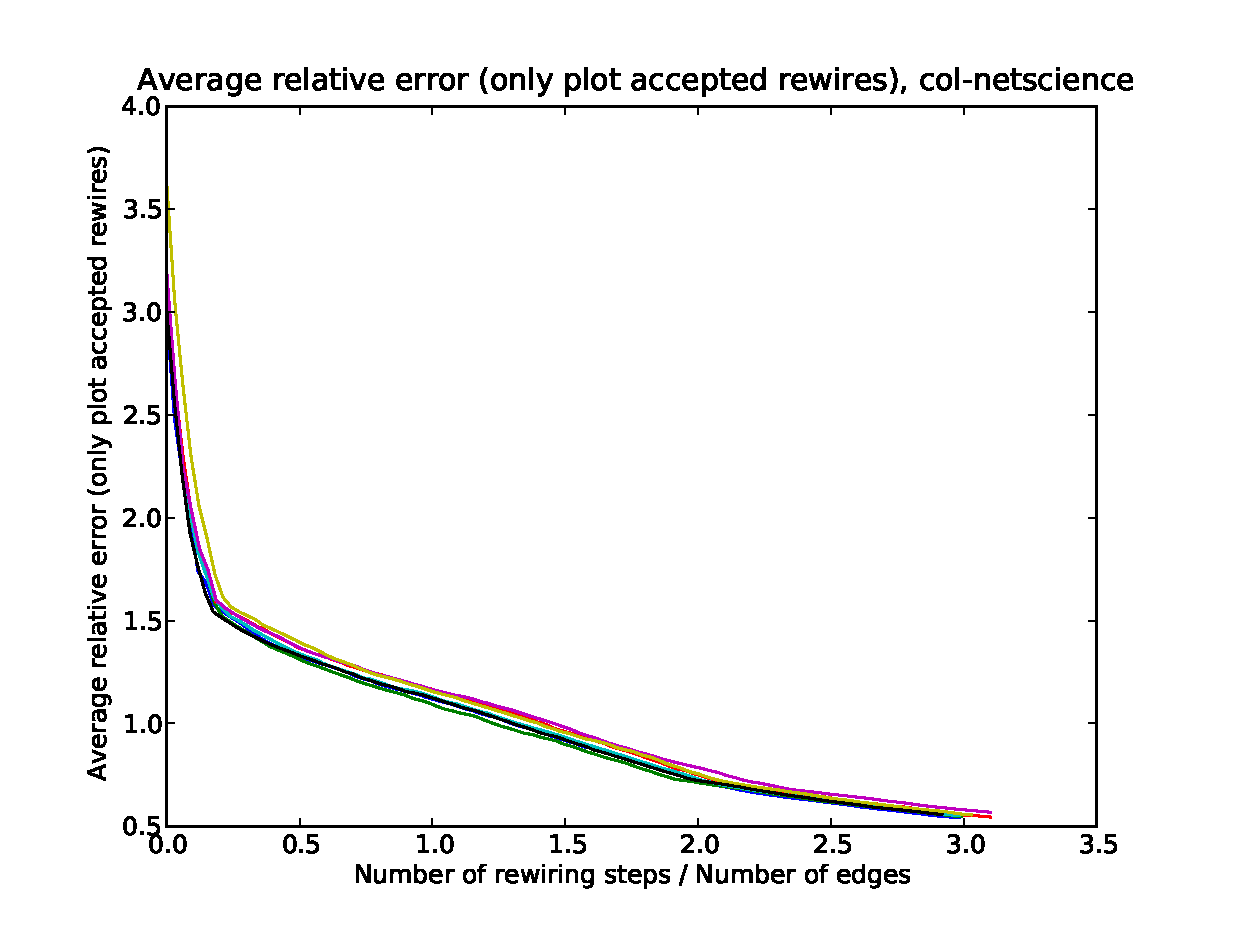
\includegraphics[width=3in]{Figures/acceptedOnly-col-netscience.eps}
\caption{Error, network col-netscience.  Only plot hill climbing steps that were successful.}
\label{fig:errors-col-netscience}
\end{figure}

\begin{figure}[p]
\centering
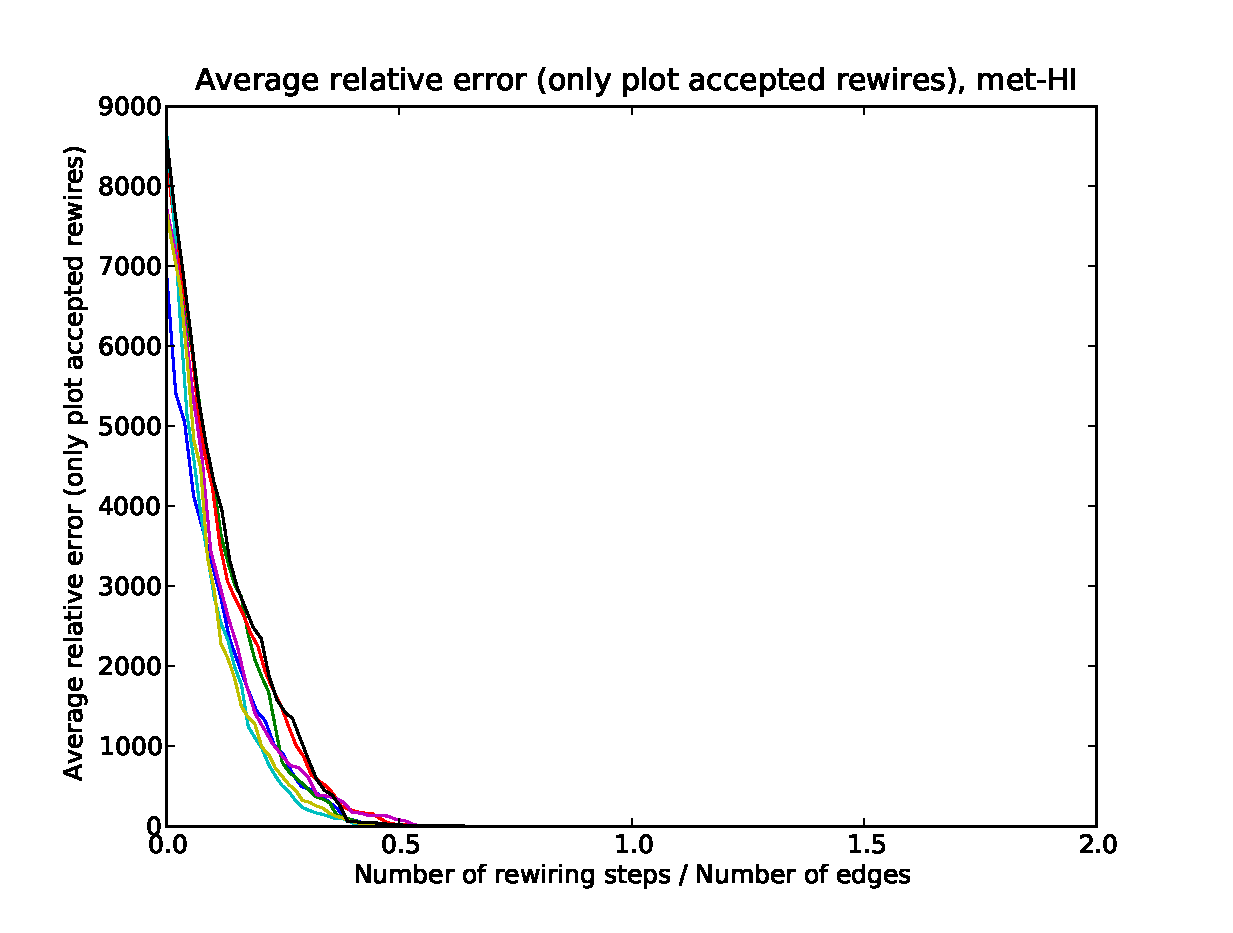
\includegraphics[width=3in]{Figures/acceptedOnly-met-HI.eps}
\caption{Error, network met-HI.  Only plot hill climbing steps that were successful.}
\label{fig:errors-met-HI}
\end{figure}

\begin{figure}[p]
\centering
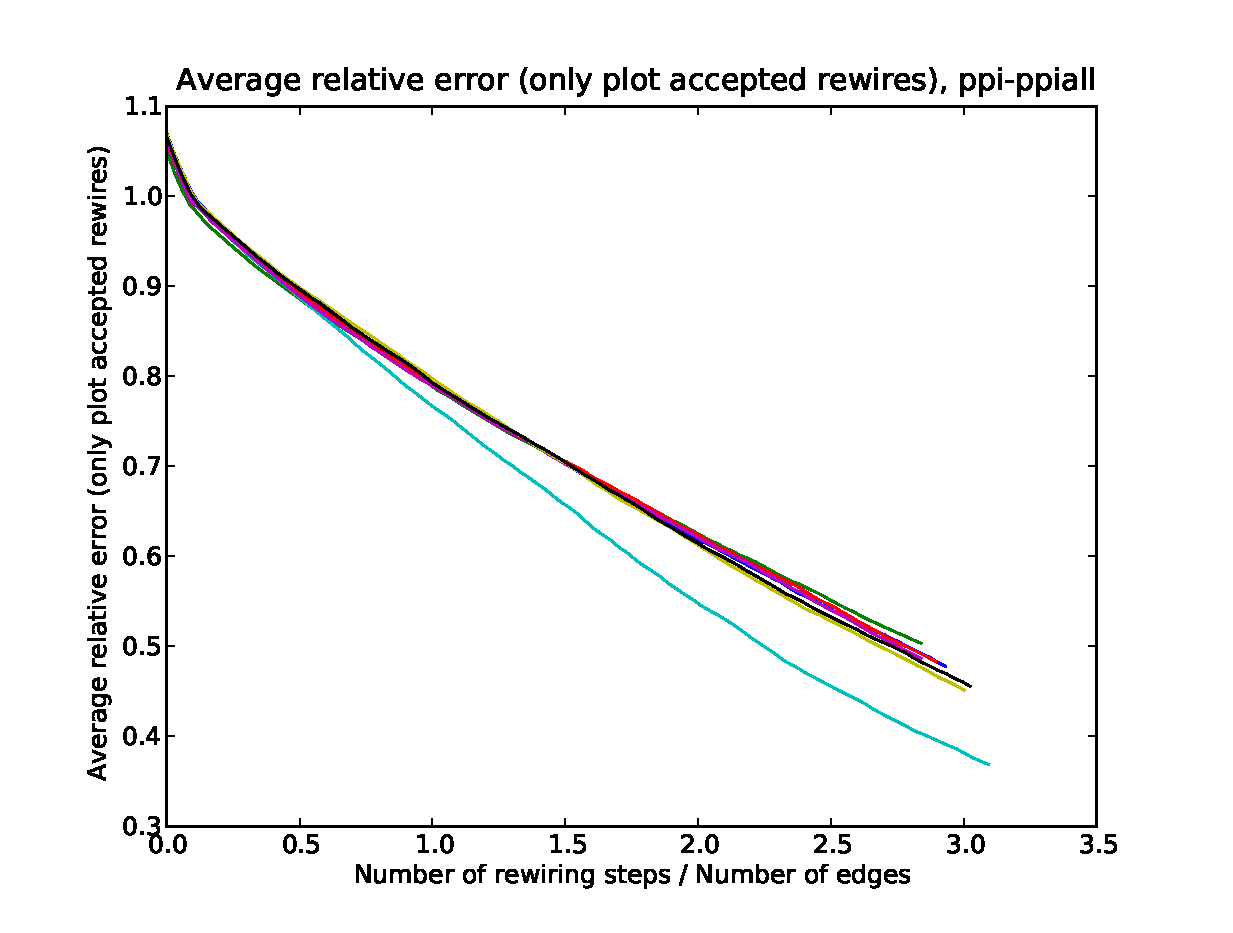
\includegraphics[width=3in]{Figures/acceptedOnly-ppi-ppiall.eps}
\caption{Error, network ppi-ppiall.  Only plot hill climbing steps that were successful.}
\label{fig:errors-ppi-ppiall}
\end{figure}

\begin{figure}[p]
\centering
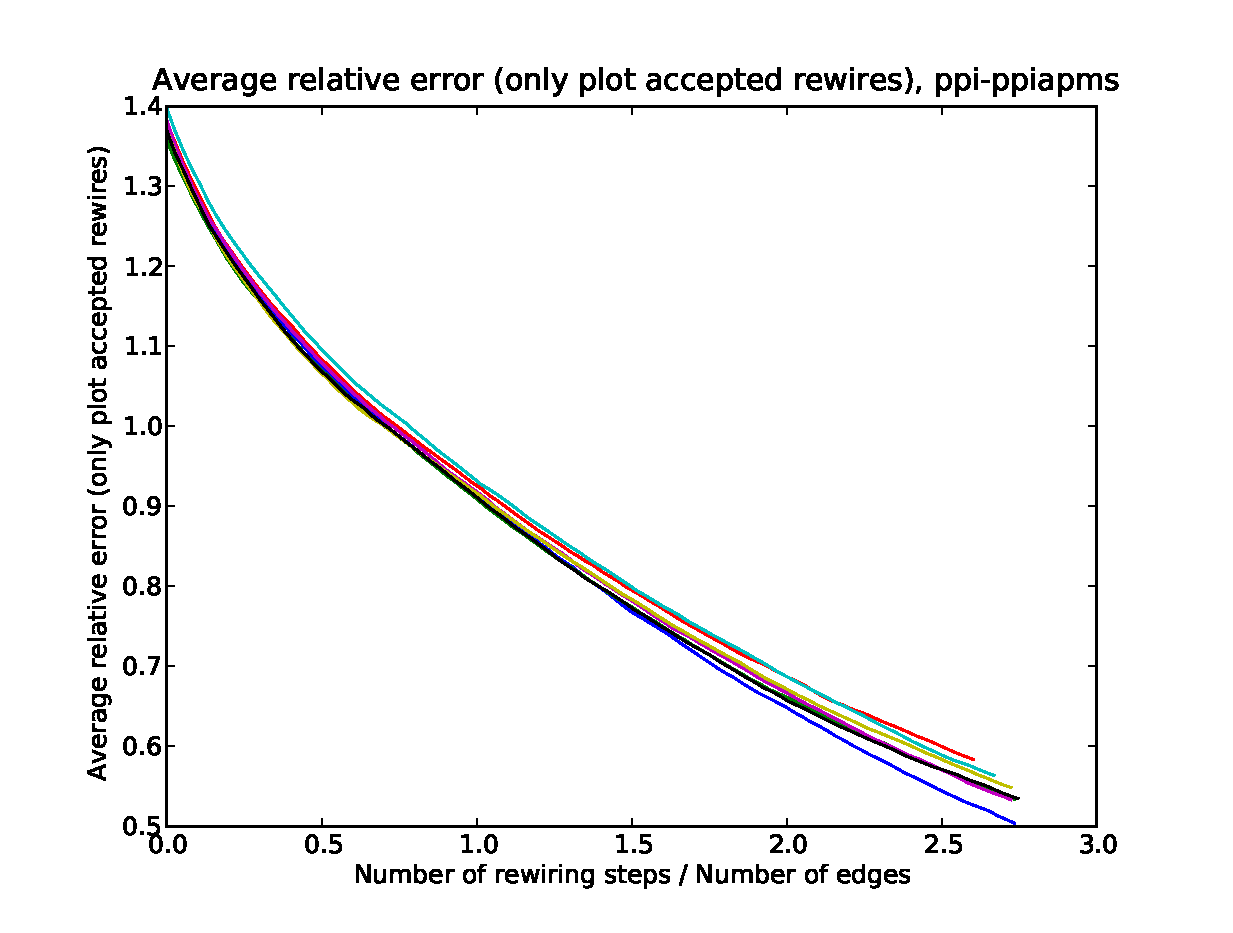
\includegraphics[width=3in]{Figures/acceptedOnly-ppi-ppiapms.eps}
\caption{Error, network ppi-ppiapms.  Only plot hill climbing steps that were successful.}
\label{fig:errors-ppi-ppiapms}
\end{figure}

\begin{figure}[p]
\centering
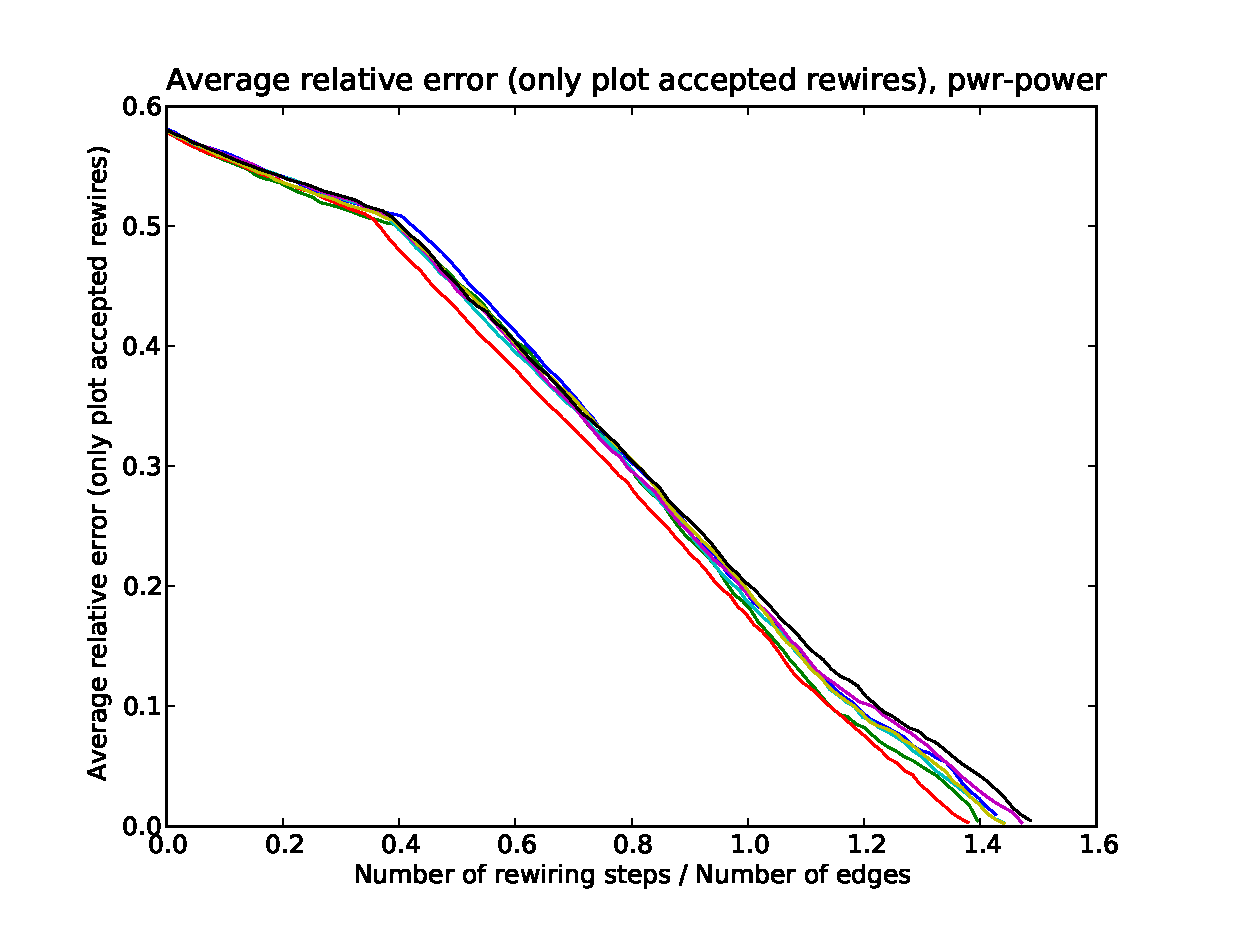
\includegraphics[width=3in]{Figures/acceptedOnly-pwr-power.eps}
\caption{Error, network pwr-power.  Only plot hill climbing steps that were successful.}
\label{fig:errors-pwr-power}
\end{figure}

\begin{figure}[p]
\centering
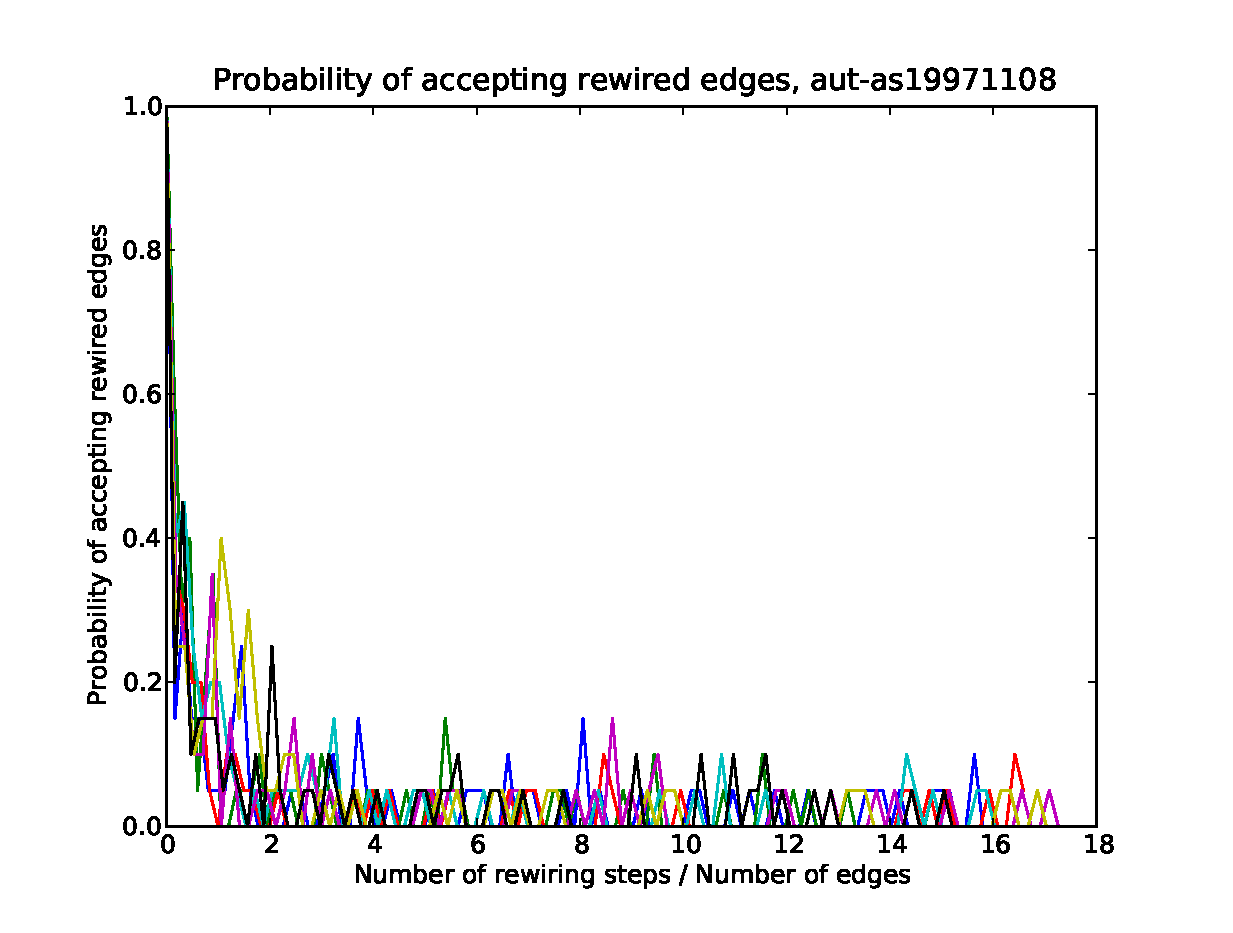
\includegraphics[width=3in]{Figures/Paccept-aut-as19971108.eps}
\caption{Probability of a rewiring step being successful, network aut-as19971108}
\label{fig:Paccept-aut-as19971108}
\end{figure}

\begin{figure}[p]
\centering
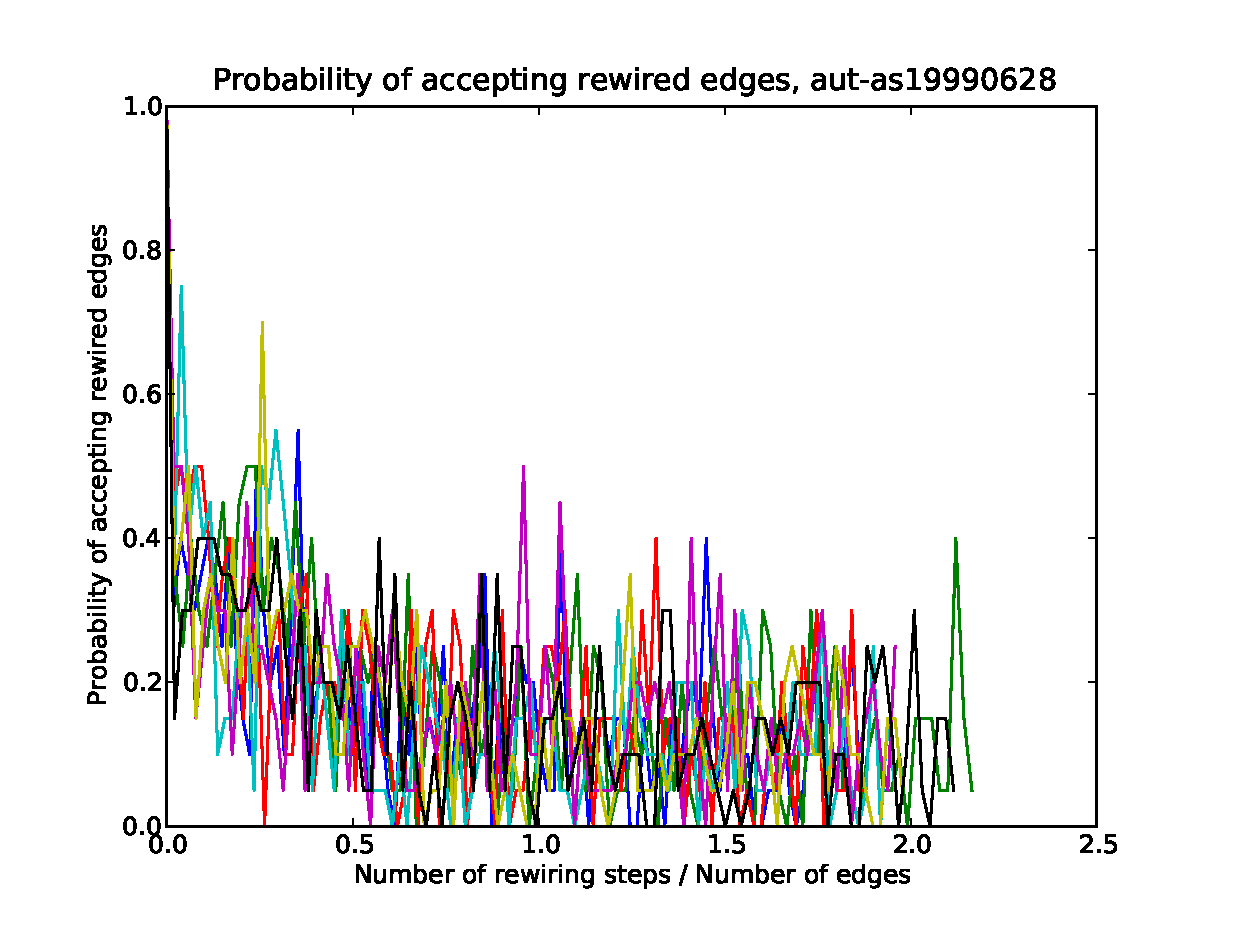
\includegraphics[width=3in]{Figures/Paccept-aut-as19990628.eps}
\caption{Probability of a rewiring step being successful, network aut-as19990628}
\label{fig:Paccept-aut-as19990628}
\end{figure}

\begin{figure}[p]
\centering
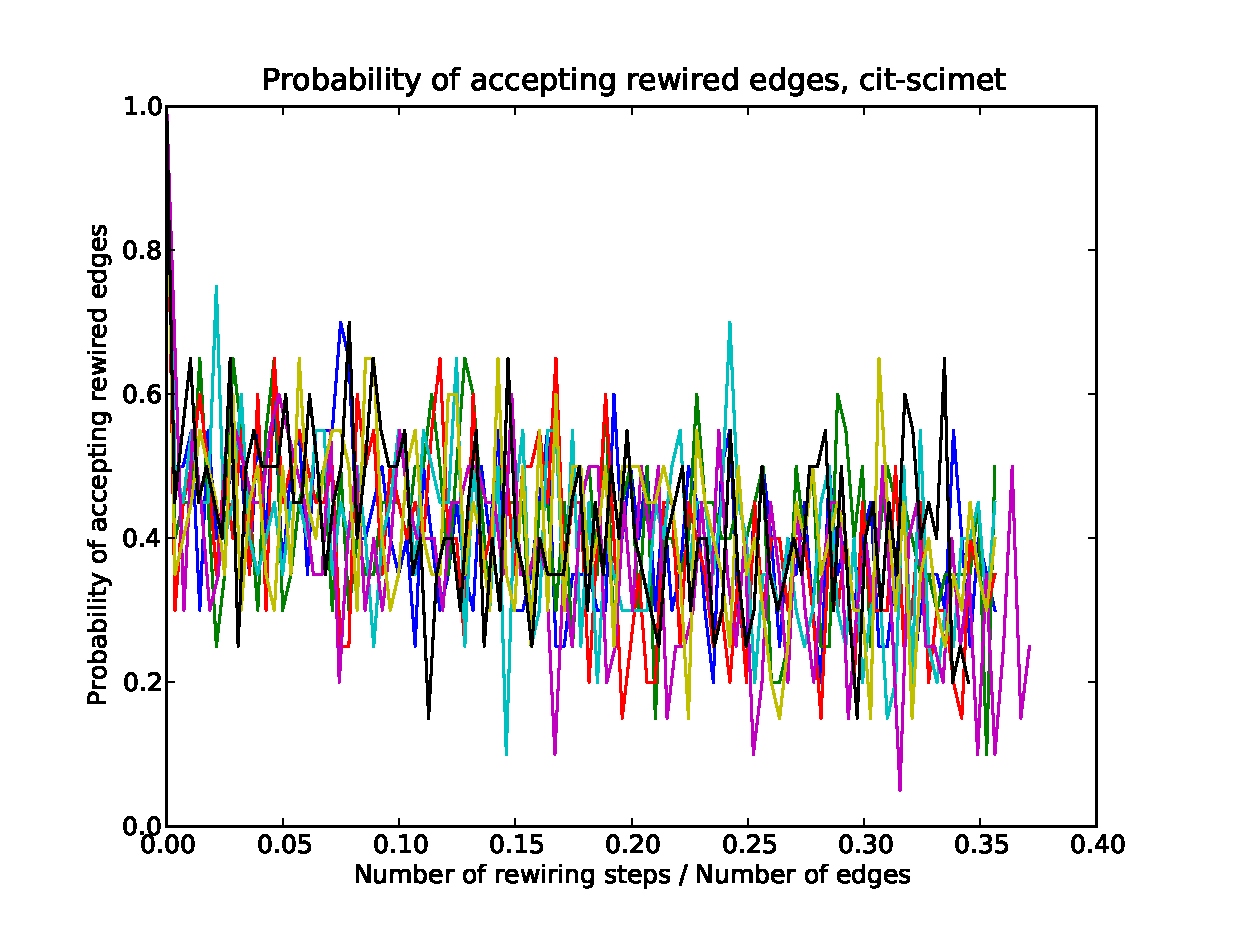
\includegraphics[width=3in]{Figures/Paccept-cit-scimet.eps}
\caption{Probability of a rewiring step being successful, network cit-scimet}
\label{fig:Paccept-cit-scimet}
\end{figure}

\begin{figure}[p]
\centering
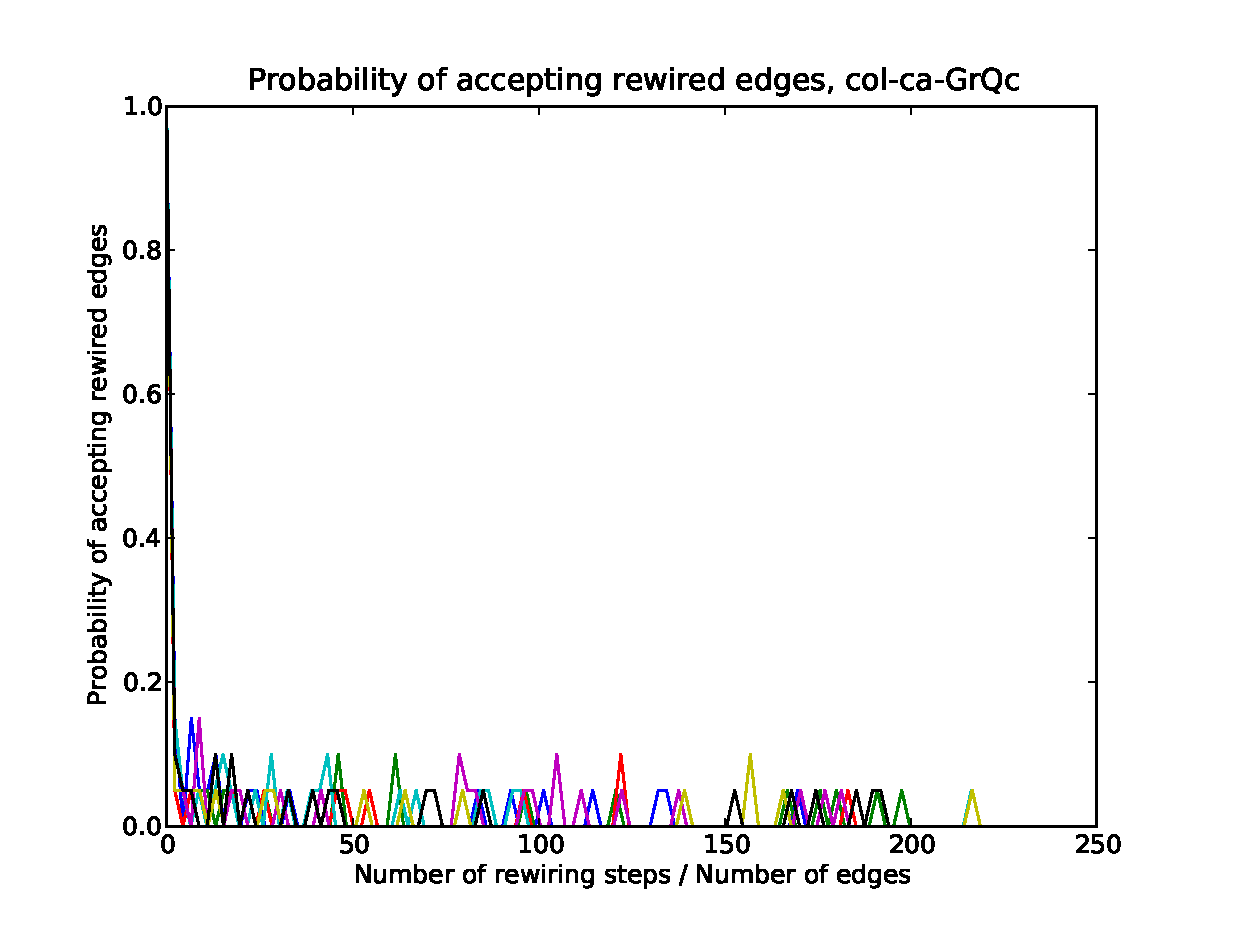
\includegraphics[width=3in]{Figures/Paccept-col-ca-GrQc.eps}
\caption{Probability of a rewiring step being successful, network col-ca-GrQc}
\label{fig:Paccept-col-ca-GrQc}
\end{figure}

\begin{figure}[p]
\centering
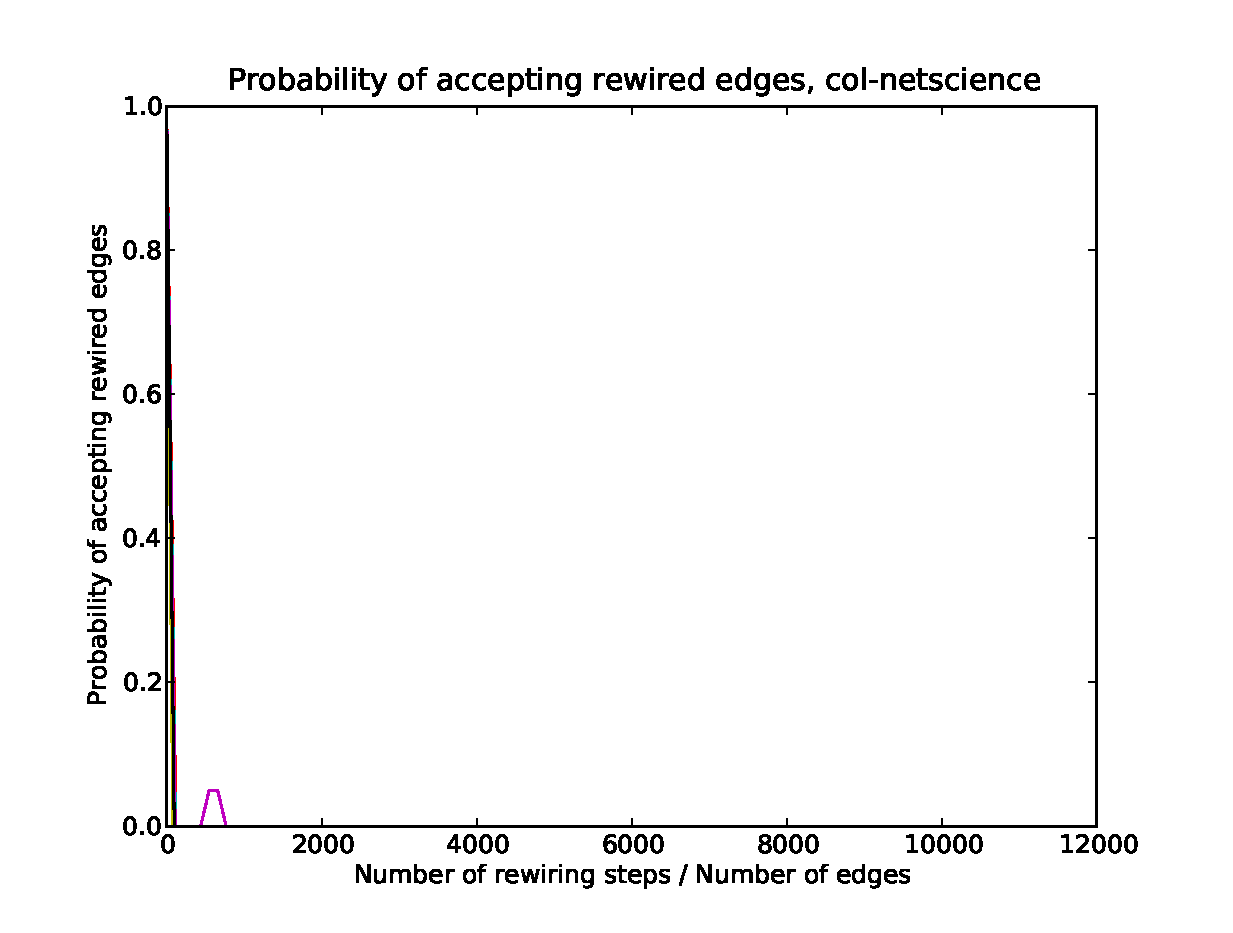
\includegraphics[width=3in]{Figures/Paccept-col-netscience.eps}
\caption{Probability of a rewiring step being successful, network col-netscience}
\label{fig:Paccept-col-netscience}
\end{figure}

\begin{figure}[p]
\centering
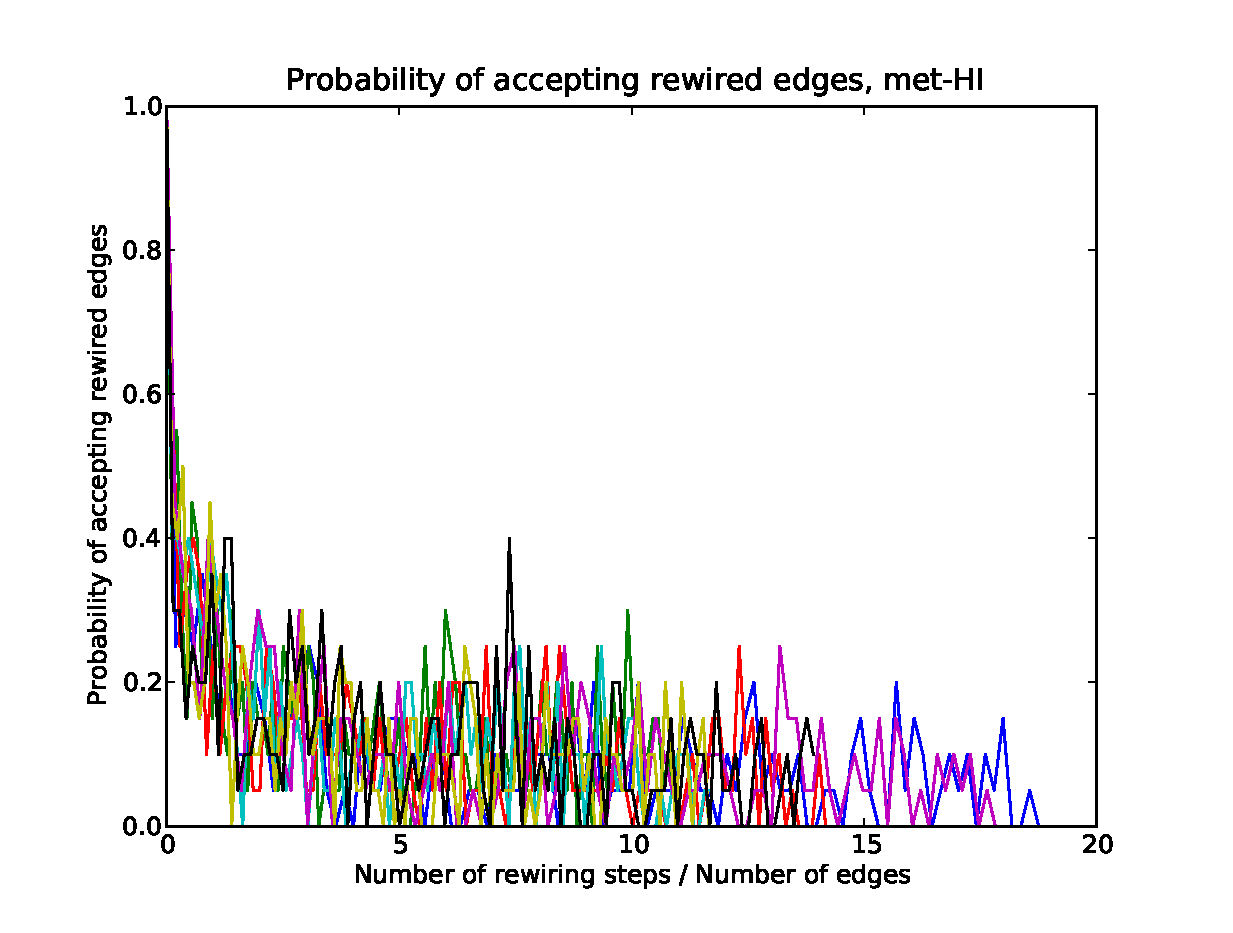
\includegraphics[width=3in]{Figures/Paccept-met-HI.eps}
\caption{Probability of a rewiring step being successful, network met-HI}
\label{fig:Paccept-met-HI}
\end{figure}

\begin{figure}[p]
\centering
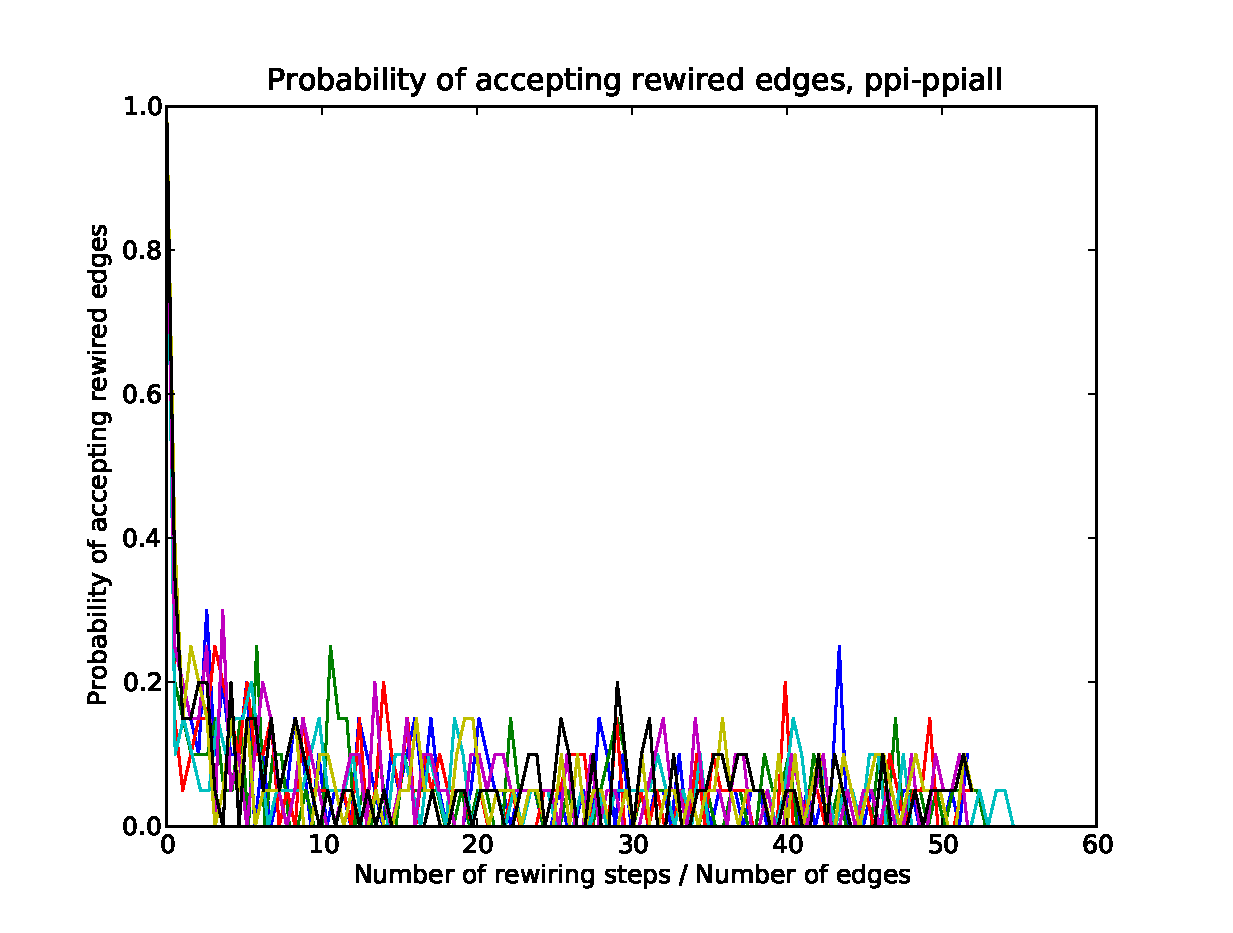
\includegraphics[width=3in]{Figures/Paccept-ppi-ppiall.eps}
\caption{Probability of a rewiring step being successful, network ppi-ppiall}
\label{fig:Paccept-ppi-ppiall}
\end{figure}

\begin{figure}[p]
\centering
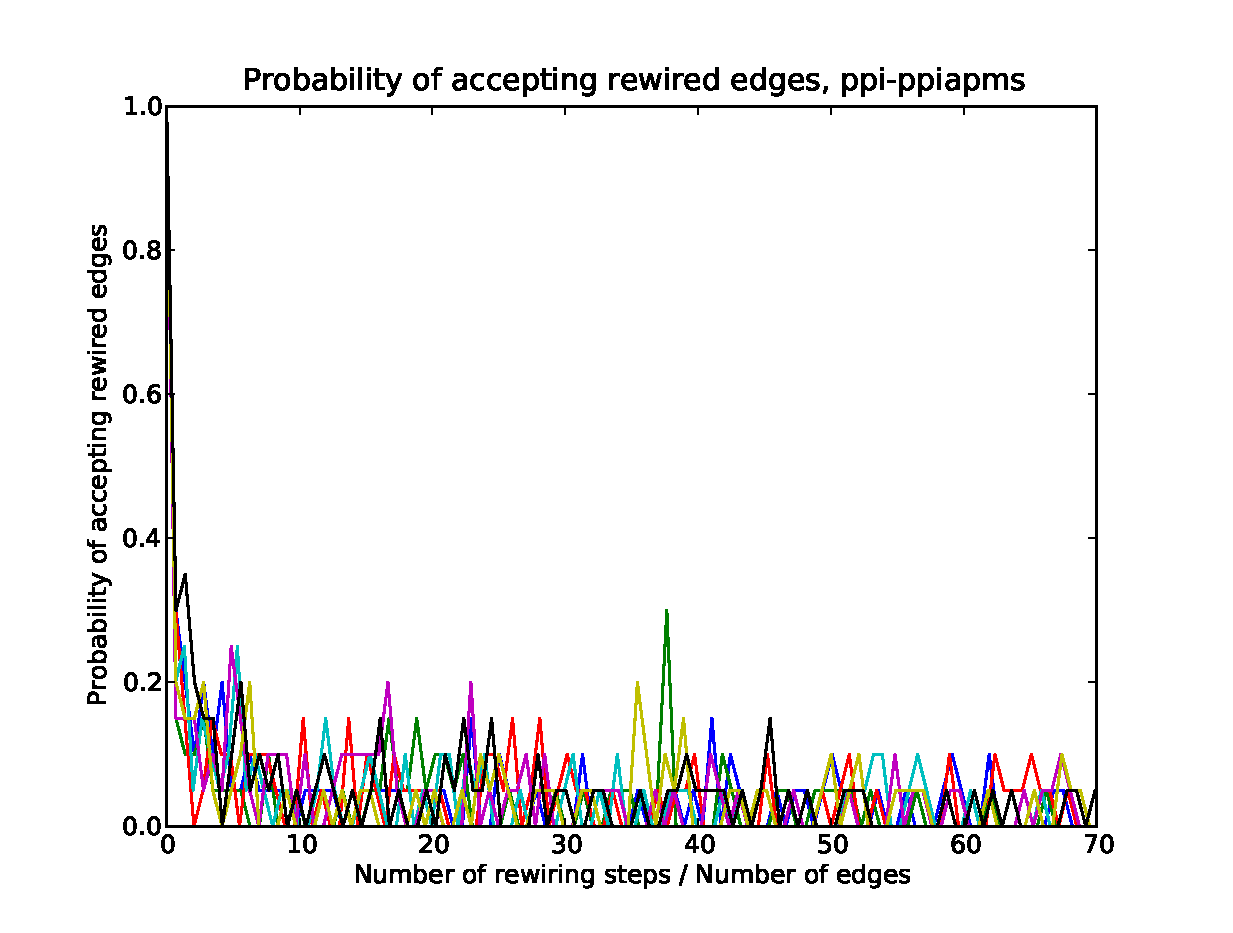
\includegraphics[width=3in]{Figures/Paccept-ppi-ppiapms.eps}
\caption{Probability of a rewiring step being successful, network ppi-ppiapms}
\label{fig:Paccept-ppi-ppiapms}
\end{figure}

\begin{figure}[p]
\centering
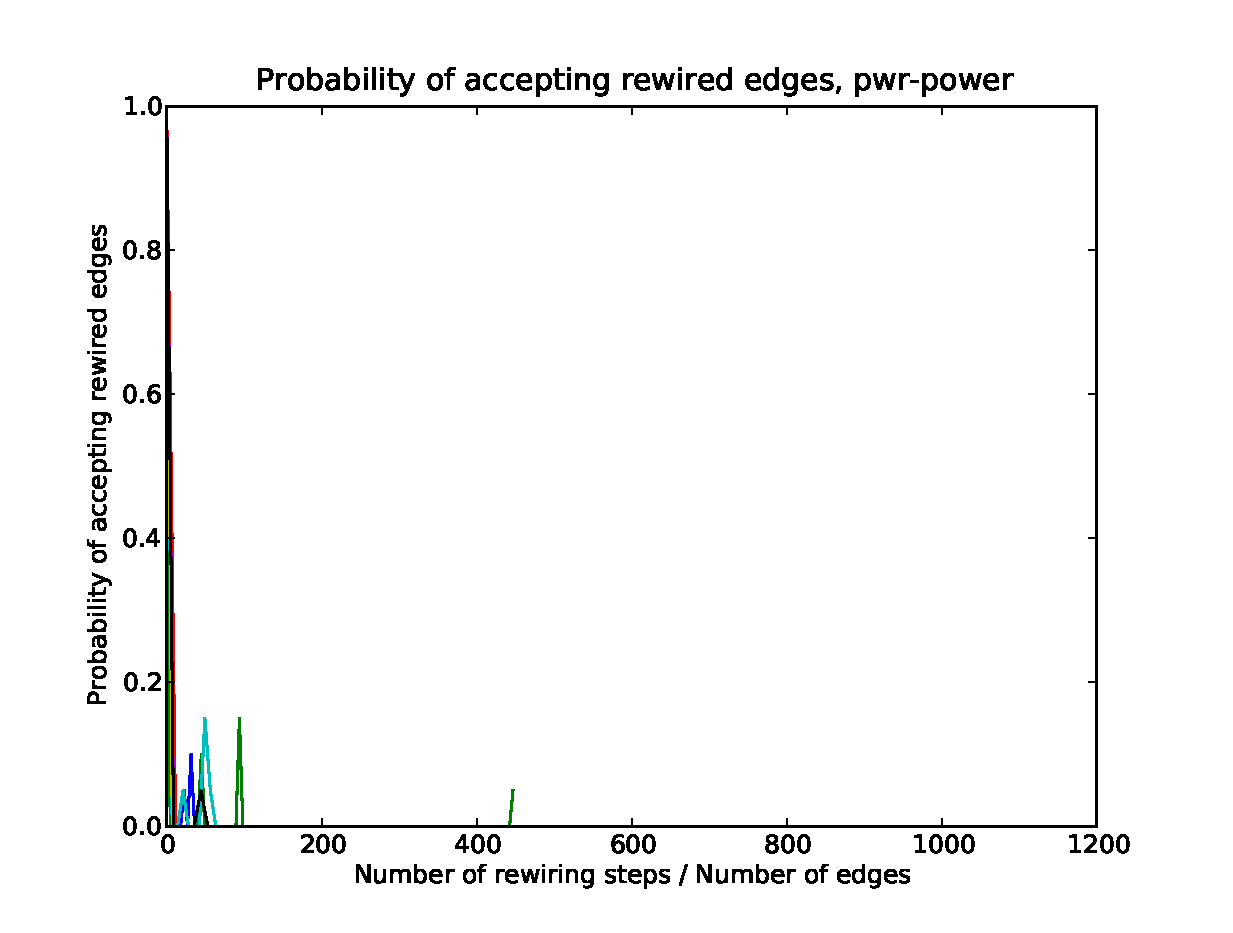
\includegraphics[width=3in]{Figures/Paccept-pwr-power.eps}
\caption{Probability of a rewiring step being successful, network pwr-power}
\label{fig:Paccept-pwr-power}
\end{figure}

\section{Predicting Degree Distribution From Motif Counts}
\label{sec:alpha}

%In this section, we present a approach framework for generating the graph. At the high level, our proposed %framework consists of two stage.
%\begin{itemize}
%    \item {\bf Degree distribution generation.} First, given a certain motif distribution, we train a gradient boosting %model using the motif distribution. And then we predict the degree distribution from motif distribution.
%    \item {\bf Candidate graph generation.} Second, with the degree distribution, we generate a random graph based %on degree distribution as candidate graph for our problem.
%    \item {\bf Graph refinement.} Second, the random graph is fed to a heuristic model to refine the graph. The model %incorporates the several strategies to refine the graph satisfied the given motif distribution.
%\end{itemize}

In previous sections we assumed that we knew the degree distribution of the graph.  Now we relax this assumption and predict the degree distribution from the motif counts.  In the future we will use this to generate graphs given only their motif counts.

We assume that all the graphs we generate have a power law degree distribution.  We use the motif counts as features to predict the power law exponent $\alpha$.  Given $\alpha$ and a normalization constant, producing an actual distribution is straightforward.

In this paper, we use Gradient Boosted Regression Trees (GBRT)~\cite{friedman2002stochastic} as the main regression model. Gradient Boosted Regression Trees is a useful machine learning method for regression problems, which is also an ensemble method that combines multiple weak prediction models. It constructs the model in a stage-wise fashion and generalizes the model by optimizing an arbitrary differentiable loss function which in our case is the square loss function
\begin{equation}
\label{eqn:loss}
\mathcal{L} = (f(x) - y)^2
\end{equation}

\noindent where $y$ is the label and $f(x)$ is our prediction for $y$.

%\footnote{Square Loss: $\mathcal{L} = (f(x) - y)^2$, here we use $\mathcal{L}$ to scribe the squared loss term, $y$ represents the label and $f(x)$ represents the predict score.}. 

More precisely, GBRT trains a lot of small tree regression models (the depth of each tree is 5), each with high bias. Instead of using a uniform weight of each model to prevent overfitting, GBRT focus on adding new trees to minimize the current remaining regression error at each iteration.Let $f(x_i)$ denote the prediction score of sample $x_i$ and $\mathcal{L}(f(x_1),...,f(x_n))$ as the loss function of the model, which reaches a minimum if $f(x_i) = y_i$ for all $x_i$. For each new tree $T_i$, that is added into the existing classifier and the current prediction $P(x_i)$, we use the following step:

$$P(x_i) \leftarrow P(x_i) + \beta \frac{\mathcal{L}}{P(x_i)}$$
\noindent where $\beta$ is the learning rate, and the gradient $\frac{\mathcal{L}}{P(x_i)}$ is approximated with the prediction score of regression tree~\cite{zheng2007general}. Algorithm~\ref{algo:gbrt} shows the details of GBRT.

\begin{algorithm}
\caption{Gradient Boosted Regression Trees (GBRT). DT indicates the decision tree model which has three parameters, data $D$, #features~f and the depth $d$ of tree.}\label{algo:gbrt}
\begin{algorithmic}
\State \textbf{Input:} Data set $\mathcal{D} =\{(x_1, y_1),..., (x_n, y_n)\}$, learning rate~\beta, \#\text{Trees}~$M$, \text{depth}~$d$ \\
\State \textbf{Output:} Combined tree model T

\State Initialization: $\forall i, p_i \leftarrow y_i$

\For {$i = 1$ to $M$} {
    $T_i \leftarrow DT(\{(x_1, p_1),..., (x_n, p_n)\}, f, d)$ \\
    \For {$j = 1$ to $n$} {
        $p_i \leftarrow p_i - \beta T_i(x_i)$\\
    }
}
$T \leftarrow \beta \sum_{i = 1}^M T_i$\\
\Return T\\
\end{algorithmic}
\end{algorithm}

\vpara{Implementation note.} In the Decision Tree model, we train $M = 1000$ trees and for each tree randomly select $f = \#\mbox{features} / 10$ and set the depth to 5. If $M$ is too big, the algorithm starts overfitting. As for learning rate, we use $\beta = 0.001$.


\hide{We use the motif distribution to predict the degree distribution.
For a given motif distribution, we use the motif distribution to predict degree distribution. The idea of this problem is using the motif distribution as a feature to train a model, and then predict a degree distribution for the given motif distribution. More precisely, we use gradient boosting as the main regression method to train a model. Gradient Boosting Tree~\cite{friedman2002stochastic} is a useful machine learning method for regression problems, which also an ensemble method with combine multiple weak prediction models. It makes the model in a stage-wise fashion and generalizes the model by optimization of the arbitrary differentiable loss function which is same as logistic regression. Here we use the python package build in~\cite{pedregosa2011scikit}. Our approach shows good performance. We achieved less than 1\% on Average Relative Error.
}

\vpara{Evaluation measures.} To quantitatively evaluate the performance of our model, we conducted experiments with different networks.  For each network, we evaluated the approach in terms of average relative error (ARE).

\vpara{Prediction performance.} We use 168 different networks as input data to evaluate the proposed model, with 10-fold cross validation. In order to avoid bias, we test the data 10 times, and get the predicted $\alpha$ for each network.  This model achieves average relative error $0.005521$ with standard deviation $0.00316$.  Some sample predictions are shown in Table~\ref{table:alpha}.

%\subsection{Candidate graph generation}
%
%According the degree distribution we got at stage 1, we use 
%
%
%=======================================
%
%
\begin{table}[t]
\centering
\label{table:alpha}
\caption{Predicted degree distribution exponents.}
\begin{tabular}{|l|l|l|l|}
\hline
Network & $\alpha$ & $\hat{\alpha}$ & Relative error\\\hline
aut-as19971108.txt & 2.53315 & 2.52657 & 0.00259 \\\hline
aut-as19990628.txt & 2.52159 & 2.54907 & -0.01090 \\\hline
cit-scimet.txt & 1.95277 & 1.93871 & 0.00720 \\\hline
col-ca-GrQc.txt & 1.88493 & 1.86740 & 0.00930 \\\hline
col-netscience.txt & 1.89612 & 1.89536 & 0.00039 \\\hline
met-HI.txt & 1.88824 &  1.87993 & 0.00439 \\\hline
ppi-ppiall.txt & 1.89357 & 1.88467 & 0.00469 \\\hline
ppi-ppiapms.txt & 1.89285 & 1.87544 & 0.00919 \\\hline
pwr-power.txt & 1.78450 &  1.78343 & 0.00059 \\\hline
\end{tabular}
\end{table}

\section{Future work}
\label{sec:futurework}



%Our current algorithms assume that we know the degree distribution of the graph.  This is fine if we have the graph of a real-world social network and we are trying to build a model to compare it to.  However, it fails if we are given the motif counts only.

%Fortunately, social networks tend to have power-law degree distributions, which means their distributions can be described by a single parameter $\alpha$, where $\alpha$ is the magnitude of the exponent.  (We also need a normalization constant, which can be found from the number of edges.)  For the final paper we will build a model to predict $\alpha$ from the motif counts.  We think we can do this because graphs with a lot of high-edge motifs should be denser, so the degree distribution should have a heavier tail.

%Models to try include linear regression, neural networks, and stochastic gradient descent.

%\section{Conclusion}
\label{sec:conclusion}


\bibliographystyle{abbrv}
\bibliography{references}  % sigproc.bib is the name of the Bibliography in this case

%\input{appendix.tex}

\end{document}

